\documentclass[11pt,a4paper]{article}

\usepackage[utf8]{inputenc}
\usepackage[expansion=false]{microtype}
\usepackage[margin=1in]{geometry}
\usepackage{amsmath,amssymb,amsthm,mathtools}
\usepackage{booktabs}
\usepackage{array}
\usepackage{multirow}
\usepackage{enumitem}
\usepackage{xcolor}
\usepackage{tikz}
\usetikzlibrary{arrows.meta,positioning,calc,backgrounds,fit,decorations.pathreplacing}
\usepackage{hyperref}

\hypersetup{
    colorlinks=true,
    linkcolor=black!80,
    citecolor=black!80,
    urlcolor=black!80,
    pdftitle={Collision and Preimage Cryptanalysis of Blender},
    pdfauthor={MiniMax}
}

\newtheorem{theorem}{Theorem}
\newtheorem{lemma}[theorem]{Lemma}
\newtheorem{proposition}[theorem]{Proposition}
\newtheorem{corollary}[theorem]{Corollary}
\theoremstyle{definition}
\newtheorem{definition}[theorem]{Definition}
\theoremstyle{remark}
\newtheorem{remark}[theorem]{Remark}

\newcommand{\F}{\mathbb{F}}
\newcommand{\Ftwo}{\mathbb{F}_2}
\newcommand{\Zmod}[1]{\mathbb{Z}/2^{#1}\mathbb{Z}}
\newcommand{\ror}{\operatorname{ror}}
\newcommand{\rol}{\operatorname{rol}}
\newcommand{\parop}{\operatorname{par}}
\newcommand{\SumAcc}{\mathsf{Sum}}
\newcommand{\Hpar}{\mathcal{H}_{\mathrm{par}}}
\newcommand{\im}{\operatorname{im}}
\newcommand{\ord}{\operatorname{ord}}
\definecolor{accent}{RGB}{165,35,35}
\definecolor{accentbg}{RGB}{250,238,238}

\title{\bfseries Collision and Preimage Cryptanalysis of Blender}
\author{MiniMax}
\date{November 2026}

\begin{document}
\maketitle

\begin{abstract}
Blender is an addition-rotation-XOR cryptographic hash function family submitted by Bradbury to the first round of the NIST SHA-3 competition in 2008. Spanning the four standard digest sizes from $224$ to $512$ bits, the algorithm pairs a carry-coupled working register and persistent carry flags with a write-only modular-sum accumulator. To resist local differentials and state-collision attacks, the design incorporates $13$-byte cyclic prefix padding, dual modular message checksums, and a minimum $32$-round block-alignment rule before discarding the working register to output the accumulator. Prior cryptanalysis required at least $2^{107.3}$ operations for preimages, lacked a practical standard-IV collision generator, and left the odd-word variant Blender-$224$ unbroken below the $2^{112}$ birthday bound.

We present a unified collision and preimage cryptanalysis of the full Blender family by exploiting the decoupling between its carry-driven working register and its write-only modular accumulator. First, we establish a global shifted subspace collapse that locks periodic register differences whenever the per-round mask count divides the state length. This reduces the $258$-bit working state of Blender-$256$ to a $38$-bit invariant graph and yields standard-IV cycle-swap collisions in under one second alongside zero-cost multicollisions. Second, we construct a local two-step differential that hides a message perturbation inside a symmetric carry transition and heals it in the next round via bitwise-complement inputs. Combined with carry-free polynomial prefix inversion and byte-lattice contraction, this trail produces constant-time semi-free-start collisions across all four NIST variants, breaks Blender-$224$ in $2^{69.56}$ evaluations, and yields minimal $24$-byte standard-IV and $36$-byte identical-prefix collisions on Blender-$256$. Third, we combine multi-shifted closed-walk steering with $2$-adic lattice invariants and generalized birthday trees over the modular accumulator ring. This reduces full first- and second-preimage complexities on Blender-$256$, Blender-$384$, and Blender-$512$ to $2^{35.93}$, $2^{66.34}$, and $2^{67.64}$ evaluations, showing that write-only modular accumulators cannot compensate for low-rank mask broadcasting.
\end{abstract}

\section{Introduction}
\label{sec:intro}

Submitted by Colin Bradbury in October~2008 and selected by NIST among the $51$ first-round SHA-3 candidates~\cite{Bra08}, Blender was designed to achieve high software throughput across $16$-, $32$-, and $64$-bit processors without lookup tables or S-boxes. A Blender instance is parameterized by a word width $w \in \{16, 32, 64\}$ in bits and a working-state length $m \in \{6, 7, 8, 9, 10\}$ in words. These parameters define a digest length $n = mw$ in bits and a per-round mask count $t \in \{2, 3\}$. The four official NIST SHA-3 variants are Blender-$224$ ($w = 32, m = 7$), Blender-$256$ ($w = 32, m = 8$), Blender-$384$ ($w = 64, m = 6$), and Blender-$512$ ($w = 64, m = 8$). All four official variants operate with $t = 2$ masks per round.

Whereas earlier stream-oriented hashes such as PANAMA~\cite{DC98} continually feed an auxiliary buffer back into the active state during absorption, Blender---like fellow first-round candidate Waterfall~\cite{Hat08}---separates its internal state into an active $m$-word working register (augmented with $t$ persistent $1$-bit carry flags) and a strictly write-only $m$-word accumulator. However, Blender's concrete compression and finalization primitives depart substantially from LFSR and S-box constructions:
\begin{enumerate}[leftmargin=2em]
    \item \textbf{Carry-Coupled ARX Compression:} At each message word, Blender evaluates $t$ modular integer additions that incorporate the persistent carry flags from the preceding step. The newly generated carry bits select a data-dependent rotation count, and the rotated sums are XORed alternately into the cyclically shifted working register.
    \item \textbf{Modular-Sum Accumulation with Working-State Truncation:} After every compression step, each updated working word is added modulo $2^w$ into the corresponding word of the write-only accumulator. The accumulator never feeds back into the working register or carry flags. At the end of finalization, the working register and carry flags are discarded, and the accumulator words are serialized to form the $n$-bit digest.
    \item \textbf{Cyclic Prefix Padding, Block Alignment, and Dual Checksums:} To counter local differentials and length-extension attacks, Blender buffers the first $13$ bytes of the message and replays them cyclically after the message body so that the message, padding, bit-length encoding, and two running modulo-$2^w$ message checksums (accumulating the absorbed words and their bitwise complements) execute at least $32$ compression rounds and end on a $16$-word block boundary before extracting the digest.
\end{enumerate}

\subsection{Prior Cryptanalysis}
After NIST accepted Blender among the $51$ first-round SHA-3 candidates in December 2008~\cite{NIST09}, six public cryptanalytic works examined the design in 2008--2009:
\begin{itemize}[leftmargin=2em]
    \item \textbf{Newbold (2008~\cite{New08}):} Newbold chained $\frac{n+w}{2} + 1$ Joux working-state collisions~\cite{Jou04} with a birthday search over the accumulator and primary checksum ($n + w$ bits). This yielded full-state collisions in $2^{(n+w)/2}$ compression rounds per stage ($2^{128}, 2^{144}, 2^{224},$ and $2^{288}$ across Blender-$224/256/384/512$---above the $2^{n/2}$ birthday bound for a single collision, but yielding $2^k$-multicollisions in $k \cdot 2^{(n+w)/2}$ rounds with $O(n)$-word segments). Applying the Gauravaram--Kelsey additive-checksum framework~\cite{GK08} yielded preimages in $n \cdot 2^{(n+w)/2}$ rounds ($2^{135.8}, 2^{152.0}, 2^{232.6},$ and $2^{297.0}$, with $O(n^2)$-word messages) using cycle-finding.
    \item \textbf{Mendel (2008~\cite{Men08}) and Lamberger--Mendel (ISC~2009~\cite{LM09}):} These works treated the compression round as a black box. By varying four message words ($4w \ge n/2$ bits) and adjusting a fifth word modulo $2^w$ to hold the five-word modular sum constant, each five-word Joux stage collides the working state and both checksums in $2^{n/2}$ evaluations (or $2^{n/2+1}$ when accounting for the two carry flags omitted in~\cite{LM09}). Repeating $n$ stages ($5n + 1$ words including a padding-adjustment word) builds a $2^n$-multicollision in published time $n \cdot 2^{n/2}$ ($2^{119.8}, 2^{136.0}, 2^{200.6},$ and $2^{265.0}$; twice as high with carry matching). A Quisquater--Delescaille memoryless meet-in-the-middle search~\cite{QD89} on the accumulator then recovers preimages across all four variants with $O(n)$ memory.
    \item \textbf{Xu and Li (IACR ePrint 2008/532~\cite{XL08}):} Xu and Li exhibited a $24$-byte ($6$-word) colliding message pair ($\mathtt{0}^4 \| \mathtt{0} \| \mathtt{ffffffff}$ versus $\mathtt{0}^4 \| \mathtt{ffffffff} \| \mathtt{0}$) exclusively for the single all-zero initial working state and zero carries. In that state, all modular additions degenerate into carry-free XORs. Because reaching the all-zero state from the standard initialization vector (IV) costs $2^{256}$ operations, no semi-free-start (SFS) generator for non-zero states or standard-IV short collision was obtained.
    \item \textbf{Kl\'{i}ma (2008~\cite{Kli08} and IACR ePrint 2009/006~\cite{Kli09}):} Kl\'{i}ma first reported a $927$-bit versus $926$-bit near-collision matching $225$ of $256$ digest bits on Blender-$256$~\cite{Kli08}. In~\cite{Kli09}, Kl\'{i}ma zeroed one mask per round in alternating order so that the $m/2$ odd-indexed working lanes repeat every $n = mw$ rounds. This left $n/2 + 2$ unconstrained bits and located $10$ working-state fixpoints in $10 \cdot n \cdot 2^{n/4 + 1}$ compression rounds ($2^{76.3}, 2^{108.9},$ and $2^{141.3}$ on Blender-$256/384/512$). Auditing~\cite{Kli09} against the Blender specification uncovers three fundamental barriers. First, although the abstract of~\cite{Kli09} claims applicability to $n = 224$, for odd $m = 7$ the cyclic register wrap-around mixes odd and even lanes and breaks periodicity completely. Second, the two-fixpoint collision construction in~\cite[Sec.~4]{Kli09} winds its first cycle $2^w$ times the second cycle length, producing colliding messages of roughly $2^{178}$ words on Blender-$256$ that require at least $2^{178}$ rounds to hash (slower than generic $2^{128}$ birthday search). Third, the multipreimage attack in~\cite[Sec.~5]{Kli09} prescribes messages of $2^{171.3}, 2^{267.3},$ and $2^{331.3}$ words on Blender-$256/384/512$. Even a minimal single-winding variant emits at least $2^{107.3}, 2^{171.9},$ and $2^{204.3}$ words, imposing an unavoidable message-hashing floor of at least $2^{107.3}$ rounds on Blender-$256$.
\end{itemize}

Prior to our work, four major cryptanalytic gaps remained open across the Blender family. First, once message-hashing costs are accounted for, no valid standard-IV collision construction faster than the $2^{n/2}$ generic birthday bound---let alone a practical sub-second collision generator---was known. Second, no collision attack faster than the $2^{112}$ birthday bound was known for odd-word Blender-$224$ ($m=7$). Third, no short ($< 100$-byte) standard-IV collision, identical-prefix collision for arbitrary prefixes, or arbitrary-state SFS generator was known for any variant. Fourth, no preimage attack broke the $2^{107}$ barrier on Blender-$256$ or the $2^{171}$ barrier on Blender-$384$ and Blender-$512$.

\begin{table}[t]
\centering
\caption{Cryptanalytic comparison across the four official NIST Blender variants ($w = 32$ for $224/256$, $w = 64$ for $384/512$; $\text{w}$ = words, $\text{B}$ = bytes, $\text{b}$ = bits; Newbold's preimage bounds appear in Table~\ref{tab:preimage-comp}). Measured runtimes are verified against the official NIST C reference~\cite{Bra08}.}
\label{tab:overview}
\footnotesize
\setlength{\tabcolsep}{3.4pt}
\renewcommand{\arraystretch}{1.04}
\begin{tabular}{@{}lllcrrr@{}}
\toprule
\textbf{Goal} & \textbf{Work} & \textbf{Setting / Mechanism} & \textbf{Var.} & \textbf{Length} & \textbf{Complexity} & \textbf{Runtime} \\
\midrule
\multirow{12}{*}{Collision}
 & Newbold~\cite{New08} & Full-state multicoll. stage & $224$ & $O(n)\text{ w}$ & $2^{128.0}$ & --- \\
 & Newbold~\cite{New08} & Full-state multicoll. stage & $256$ & $O(n)\text{ w}$ & $2^{144.0}$ & --- \\
 & Newbold~\cite{New08} & Full-state multicoll. stage & $384$ & $O(n)\text{ w}$ & $2^{224.0}$ & --- \\
 & Newbold~\cite{New08} & Full-state multicoll. stage & $512$ & $O(n)\text{ w}$ & $2^{288.0}$ & --- \\
 & Kl\'{i}ma~\cite{Kli09} & Odd-lane fixpoint winding & $256$ & $2^{178.0}\text{ w}$ & $\ge 2^{178.0}$ & --- \\
 & Kl\'{i}ma~\cite{Kli09} & Odd-lane fixpoint winding & $384$ & $2^{275.0}\text{ w}$ & $\ge 2^{275.0}$ & --- \\
 & Kl\'{i}ma~\cite{Kli09} & Odd-lane fixpoint winding & $512$ & $2^{340.0}\text{ w}$ & $\ge 2^{340.0}$ & --- \\
 & \textbf{Ours (\S\ref{sec:route2})} & Silent carry healing & $\mathbf{224}$ & $\mathbf{6\text{ w}}$ & $\mathbf{2^{69.56}}$ & --- \\
 & \textbf{Ours (\S\ref{sec:route1})} & Clean-subspace cycle swap & $\mathbf{256}$ & $4{,}000\text{ w}$ & $2^{22.60}$ & $\mathbf{0.73\text{ s}}$ \\
 & \textbf{Ours (\S\ref{sec:route2})} & Global-min carry healing & $\mathbf{256}$ & $\mathbf{6\text{ w}}$ & --- & $\mathbf{34.6\text{ s}}$ \\
 & \textbf{Ours (\S\ref{sec:route1})} & Clean-subspace cycle swap & $\mathbf{384}$ & $4{,}096\text{ w}$ & $\mathbf{2^{57.60}}^{\mathrm{a}}$ & --- \\
 & \textbf{Ours (\S\ref{sec:route1})} & Clean-subspace cycle swap & $\mathbf{512}$ & $4{,}096\text{ w}$ & $\mathbf{2^{58.00}}^{\mathrm{a}}$ & --- \\
\midrule
\multirow{8}{*}{\shortstack[l]{SFS /\\Short}}
 & Kl\'{i}ma~\cite{Kli08} & $225/256$-bit near-collision & $256$ & $927\text{ b}$ & --- & --- \\
 & Xu--Li~\cite{XL08} & Zero-state SFS only & $256$ & $24\text{ B}$ & $O(1)$ & --- \\
 & \textbf{Ours (\S\ref{sec:route2})} & Closed-form arbitrary SFS & $\mathbf{224}$ & $113\text{ B}$ & $O(1)$ & $\mathbf{0.027~\mu\text{s}}$ \\
 & \textbf{Ours (\S\ref{sec:route2})} & Closed-form arbitrary SFS & $\mathbf{256}$ & $113\text{ B}$ & $O(1)$ & $\mathbf{0.006~\mu\text{s}}$ \\
 & \textbf{Ours (\S\ref{sec:route2})} & Closed-form arbitrary SFS & $\mathbf{384}$ & $229\text{ B}$ & $O(1)$ & $\mathbf{0.054~\mu\text{s}}$ \\
 & \textbf{Ours (\S\ref{sec:route2})} & Closed-form arbitrary SFS & $\mathbf{512}$ & $229\text{ B}$ & $O(1)$ & $\mathbf{0.014~\mu\text{s}}$ \\
 & \textbf{Ours (\S\ref{sec:route2})} & Identical-prefix ($3$R steer) & $\mathbf{256}$ & $\mathbf{36\text{ B}}$ & --- & ---$^{\mathrm{b}}$ \\
 & \textbf{Ours (\S\ref{sec:route2})} & Identical-prefix ($4$R lattice) & $\mathbf{256}$ & $40\text{ B}$ & --- & $\mathbf{145.5\text{ s}}$ \\
\midrule
\multirow{10}{*}{Preimage}
 & Lamberger--Mendel~\cite{LM09} & $5$-word sum-fixed Joux & $224$ & $1{,}121\text{ w}$ & $2^{119.81}$ & --- \\
 & Lamberger--Mendel~\cite{LM09} & $5$-word sum-fixed Joux & $256$ & $1{,}281\text{ w}$ & $2^{136.00}$ & --- \\
 & Kl\'{i}ma~\cite{Kli09} & Multipreimage winding & $256$ & $2^{107.3}\text{ w}$ & $\ge 2^{107.32}$ & --- \\
 & \textbf{Ours (\S\ref{sec:dsos})} & Multi-shifted Wagner $k$-tree & $\mathbf{256}$ & $2^{27.46}\text{ w}$ & $\mathbf{2^{35.93}}$ & --- \\
 & Lamberger--Mendel~\cite{LM09} & $5$-word sum-fixed Joux & $384$ & $1{,}921\text{ w}$ & $2^{200.58}$ & --- \\
 & Kl\'{i}ma~\cite{Kli09} & Multipreimage winding & $384$ & $2^{171.9}\text{ w}$ & $\ge 2^{171.90}$ & --- \\
 & \textbf{Ours (\S\ref{sec:dsos})} & Multi-shifted Wagner $k$-tree & $\mathbf{384}$ & $2^{38.91}\text{ w}$ & $\mathbf{2^{66.34}}$ & --- \\
 & Lamberger--Mendel~\cite{LM09} & $5$-word sum-fixed Joux & $512$ & $2{,}561\text{ w}$ & $2^{265.00}$ & --- \\
 & Kl\'{i}ma~\cite{Kli09} & Multipreimage winding & $512$ & $2^{204.3}\text{ w}$ & $\ge 2^{204.32}$ & --- \\
 & \textbf{Ours (\S\ref{sec:dsos})} & Multi-shifted Wagner $k$-tree & $\mathbf{512}$ & $2^{39.25}\text{ w}$ & $\mathbf{2^{67.64}}$ & --- \\
\bottomrule
\addlinespace[2pt]
\multicolumn{7}{@{}l@{}}{\scriptsize $^{\mathrm{a}}$At $4{,}096$-word cap ($\approx 2^{34.8}$ rounds unconstrained).\quad $^{\mathrm{b}}$Explicit $36$-byte witness verified in Table~\ref{tab:short-witnesses}.}
\end{tabular}
\end{table}

\subsection{Our Contributions and Technical Overview}
Table~\ref{tab:overview} summarizes our results across the Blender family. Our analysis develops three core techniques:
\begin{enumerate}[leftmargin=2em]
    \item \textbf{Shifted Clean Subspace Collapse, Parity Obstruction, and Sub-Second Cycle-Swap Collisions (Section~\ref{sec:route1}):} Across all $15$ variants in Bradbury's specification, we prove a general divisibility criterion for subspace closure. Constraining the leading updated working word to a constant word or its bitwise complement makes all $m - t$ stride-$t$ register XOR differences message-independent if and only if $t$ divides $m$. This criterion holds for $9$ of the $15$ variants (including Blender-$256$, Blender-$384$, and Blender-$512$) and explains why odd-lane periodicity fails on $7$-word Blender-$224$. On Blender-$256$, our construction collapses Kl\'{i}ma's $130$-bit alternating state~\cite{Kli09} to a $38$-bit period-$8$ clean subspace ($2^{92}$ times smaller). We also establish a Parity Obstruction Theorem proving that the unshifted zero-difference fixed point is unreachable from the standard Blender-$256$ IV for any message. In addition, we prove that the carry-coupled branching graph on the clean subspace has an exact mean out-degree of $2.000$. Pairing two overlapping ancestor cycles on a single depth-first search (DFS) tree yields standard-IV Blender-$256$ collisions in $0.045\text{--}0.73$~s, zero-cost $\binom{2r}{r}$ multicollisions, and $\Theta(2^w/\ell)$ collisions on Blender-$384$ and Blender-$512$.
    \item \textbf{Two-Step Silent Carry Healing, All-Variant $O(1)$ SFS, and Solver-Free $24$-Byte Collisions (Section~\ref{sec:route2}):} Bypassing the $t \mid m$ divisibility barrier via a two-step local perturbation-and-correction trail~\cite{CJ98}, we introduce a carry-coupled ARX differential. The first step injects a silent carry perturbation that leaves the working register and accumulator unchanged while flipping both carry flags from $(0,0)$ to $(1,1)$. The second step applies bitwise-complement message words that lock the adder inputs to mid-point constants, simultaneously healing the carry difference and preserving both modular message checksums. We establish an unordered state validity density of $2^{-69.56}$ across Blender-$224$ and $2^{-69.58}$ across Blender-$256$, breaking Blender-$224$ in $2^{69.56} \ll 2^{112}$ state evaluations. We also derive deterministic zero-retry $O(1)$ closed-form SFS collisions for all four NIST variants via circulant polynomial inversion, and prove that $24$ bytes ($6$ words) is the global minimum standard-IV collision length on Blender-$256$. Finally, we build a solver-free $4$-round lane-invariant and $2$-round byte-lattice contraction solver ($0.11\text{--}0.29$~ms per target) that finds $24$-byte standard-IV and $40$-byte identical-prefix collisions in pure C.
    \item \textbf{Multi-Shifted Closed-Walk Steering and Preimage Cryptanalysis (Section~\ref{sec:dsos}):} Building on multi-block internal-state collisions~\cite{Jou04} and generalized birthday checksum cancellation~\cite{Wag02,GK08,MPRKS08}, we develop a multi-shifted closed-walk preimage attack over the modular ring of Blender's accumulator. Because Blender discards its working state immediately after the checksum rounds, equal-length, equal-checksum closed walks require no finalization inversion. Using $2$-adic Smith Normal Form (SNF) analysis, we show that unshifted clean walks suffer a $12$-bit subgroup rank defect that starves the leading accumulator lane. We prove that chaining closed walks across multiple shifted clean subspaces injects odd $2$-adic units into the leading lane and saturates the maximal parity subgroup of index $2^{m-2}$. Combining $8$-anchor reverse-reachable DAG~\cite{KK06} slot generation with a joint checksum-and-accumulator generalized birthday tree~\cite{Wag02} reduces full first- and second-preimage complexities to $2^{35.93}$ on Blender-$256$, $2^{66.34}$ on Blender-$384$, and $2^{67.64}$ on Blender-$512$. We also verify the exact $2$-adic SNF subgroup ranks and the closed-walk modular superposition identity empirically on Bradbury's unmodified NIST C reference implementation.
\end{enumerate}

\subsection{Paper Organization}
Section~\ref{sec:spec} establishes our algebraic notation, circulant polynomial and $2$-adic lattice preliminaries, and the complete mathematical specification of the Blender family. Section~\ref{sec:route1} develops our shifted clean subspace collapse, the Parity Obstruction Theorem, and the single-stage overlapping cycle-swap collision and multicollision attacks. Section~\ref{sec:route2} presents our two-step silent carry injection and complement healing trail, closed-form SFS generators for all four NIST variants, and solver-free $24$-byte standard-IV and identical-prefix collision attacks. Section~\ref{sec:dsos} introduces multi-shifted modular-sum steering, proves the $2$-adic SNF subgroup hierarchy, and derives our full first- and second-preimage attacks. Section~\ref{sec:eval} summarizes the root architectural vulnerabilities and reports experimental verification benchmarks and concrete witnesses.

\section{Preliminaries and Specification}
\label{sec:spec}

\subsection{Notation and Algebraic Preliminaries}
\label{subsec:prelim}
Throughout this paper, $w \in \{16, 32, 64\}$ denotes the word bit-width and $b = w/8 \in \{2, 4, 8\}$ denotes the byte length of a word. We write $\Ftwo = \mathbb{Z}/2\mathbb{Z}$ for the binary field and $\Zmod{w}$ for the residue ring of integers modulo $2^w$.

\paragraph{Bitwise and Modular Word Operations.}
We identify the set of $w$-bit words $\{0,1\}^w$ with the integer interval $\{0, 1, \dots, 2^w - 1\}$ via the little-endian binary expansion $z = \sum_{j=0}^{w-1} z_{[j]}\,2^j$, where $z_{[j]} \in \Ftwo$ denotes bit~$j$ of $z$. For any $w$-bit word $z$, its bit-parity is $\parop(z) \coloneqq \bigoplus_{j=0}^{w-1} z_{[j]} \in \Ftwo$, and its $j$-th little-endian byte ($0 \le j < b$) is $\mathrm{byte}_j(z) \coloneqq \lfloor z / 2^{8j} \rfloor \bmod 2^8$. We write $\mathbf{0}$ for the all-zero word (or all-zero tuple), $\mathbf{1} \coloneqq 2^w - 1$ for the all-ones word, $x \oplus y$ for bitwise XOR, and $\neg x \coloneqq x \oplus \mathbf{1} = (2^w - 1) - x$ for bitwise complement. For any integer $k$, $\ror_k(x)$ and $\rol_k(x)$ denote $w$-bit right and left cyclic rotations by $k \bmod w$ bit positions. We write $x \boxplus y = (x + y) \bmod 2^w$ and $x \boxminus y = (x - y) \bmod 2^w$ for addition and subtraction in $\Zmod{w}$, extended componentwise to the $m$-word abelian group $\mathcal{G} \coloneqq (\Zmod{w})^m$. For a byte or word sequence $U$, we denote its length by $|U|$ (or $\ell(U)$), write $U \| V$ for concatenation, and write $\mathbf{1}[\mathcal{E}] \in \{0,1\}$ for the indicator of event $\mathcal{E}$.

\paragraph{Circulant Polynomial Representation.}
Each $w$-bit word $z \in \Ftwo^w$ with bits $(z_{[0]}, \dots, z_{[w-1]})$ corresponds bijectively to the polynomial $z(X) = \sum_{j=0}^{w-1} z_{[j]}\,X^j$ in the quotient ring $\mathcal{R}_w \coloneqq \Ftwo[X]/(X^w + 1)$. Since $X^w = 1$ in $\mathcal{R}_w$, cyclic left rotation $\rol_k(z)$ acts as multiplication by $X^{k \bmod w}$, and cyclic right rotation $\ror_k(z)$ acts as multiplication by $X^{(w - k) \bmod w}$. Any $\Ftwo$-linear combination of cyclic rotations $L(z) = \bigoplus_{k \in S} \rol_k(z)$ corresponds to multiplication by the circulant polynomial $f(X) = \sum_{k \in S} X^k \in \mathcal{R}_w$. Because $w = 2^e$ is a power of two, $(X^w + 1) = (X + 1)^{2^e}$ over $\Ftwo$, so $f(X)$ is invertible in $\mathcal{R}_w$ if and only if $f(1) \equiv |S| \equiv 1 \pmod 2$ (odd Hamming weight). Whenever $f(1) = 1$, we have $f(X)^{2^e} = f(X^{2^e}) = f(1) = 1$ in $\mathcal{R}_w$, giving the closed-form inverse $f(X)^{-1} = \prod_{j=0}^{e-1} f(X)^{2^j}$ in $\mathcal{R}_w$ via $e = \log_2 w$ squarings.

\paragraph{Two-Adic Valuation and Smith Normal Form.}
For any integer $z \in \mathbb{Z}$, the $2$-adic valuation $\nu_2(z)$ is the largest exponent $v \ge 0$ such that $2^v$ divides $z$, with $\nu_2(0) \coloneqq w$ on $\Zmod{w}$. An element $u \in \Zmod{w}$ is a $2$-adic unit (invertible modulo $2^w$) if and only if $\nu_2(u) = 0$, that is, $u$ is odd. Over the local principal ideal ring $\Zmod{w}$, any subgroup ($\Zmod{w}$-submodule) $\mathcal{H} \le \mathcal{G} = (\Zmod{w})^m$ generated by a family of difference vectors admits a $2$-adic Smith Normal Form (SNF) decomposition via unimodular row and column operations. Its invariant factors take the form $(d_0, d_1, \dots, d_{m-1}) = (2^{v_0}, 2^{v_1}, \dots, 2^{v_{m-1}})$ with non-decreasing $2$-adic valuations $0 \le v_0 \le v_1 \le \dots \le v_{m-1} \le w$. Consequently, $\mathcal{H} \cong \bigoplus_{i=0}^{m-1} 2^{v_i}(\Zmod{w})$ has finite index $[\mathcal{G} : \mathcal{H}] = \prod_{i=0}^{m-1} d_i = 2^{\sum_{i=0}^{m-1} v_i}$ and bit codimension $\sum_{i=0}^{m-1} v_i$ inside $(\Zmod{w})^m$.

\subsection{State Layout and Initialization}
\label{subsec:spec-init}
We follow the official NIST SHA-3 Round-1 specification and C/C++ reference submission~\cite{Bra08}. Blender defines $15$ hash instances indexed by word width $w \in \{16, 32, 64\}$ and state word count $m \in \{6, 7, 8, 9, 10\}$, producing an $n = mw$-bit digest. The per-round mask count is $t = 2$ for $m \in \{6, 7, 8\}$ (the \emph{$x2$ family}, which encompasses all four required NIST SHA-3 output sizes) and $t = 3$ for $m \in \{9, 10\}$ (the \emph{$x3$ family}):
\[
    \text{Blender-}224: (w{=}32, m{=}7, t{=}2), \quad
    \text{Blender-}256: (w{=}32, m{=}8, t{=}2),
\]
\[
    \text{Blender-}384: (w{=}64, m{=}6, t{=}2), \quad
    \text{Blender-}512: (w{=}64, m{=}8, t{=}2).
\]
Each Blender instance maintains six state components. The active trunk consists of working words $W = (W_0, \dots, W_{m-1}) \in (\{0,1\}^w)^m$ and persistent carry flags $c_1, c_2 \in \{0,1\}$ (plus $c_3 \in \{0,1\}$ when $t = 3$). The output and schedule state consists of modular-sum accumulators $\SumAcc = (\SumAcc[0], \dots, \SumAcc[m-1]) \in (\Zmod{w})^m$, running word checksums $C_1, C_2 \in \Zmod{w}$, a $13$-byte prefix buffer $F[0 \dots 12]$, and a fragment-alignment counter enforcing the $32$-round minimum and $16$-fragment block alignment.

At initialization, $\SumAcc = (0, \dots, 0)$, $c_1 = c_2 = 0$, and $C_1 = C_2 = 0$. The initial working words $W^{\mathrm{IV}}$ are derived from fractional square roots of primes (matching the standard initial words of SHA-$224$, SHA-$256$, and SHA-$512$ for Blender-$224$, Blender-$256$, and Blender-$512$). In Bradbury's official NIST C/C++ reference implementation~\cite{Bra08}, the Blender-$384$ ($m=6$) initialization loop loads five $64$-bit words and leaves $W^{\mathrm{IV}}_5 = 0$ rather than loading a sixth table entry (whereas Blender-$224$ copies eight entries from an $18$-word table whose first seven entries match SHA-$224$, leaving the eighth slot unused). All structural theorems, closed-form SFS generators, out-degree laws, and preimage bounds in this paper hold identically under both the written specification IVs and the official C reference IVs. All concrete digests and test witnesses are verified directly against the unmodified NIST C reference.

\subsection{Compression Round and Carry Coupling}
\label{subsec:spec-round}
Message bytes are absorbed in little-endian $w$-bit fragments $f_k = \sum_{j=0}^{b-1} \mathrm{byte}_{bk+j}\,2^{8j} \in \{0,1\}^w$. For each absorbed fragment $f_k$ during message, prefix-pad, and length absorption (prior to the checksum words), the running checksums update via
\begin{equation}
    C_1 \leftarrow (C_1 + f_k) \bmod 2^w, \qquad C_2 \leftarrow (C_2 + \neg f_k) \bmod 2^w.
    \label{eq:checksums}
\end{equation}
After $L$ absorbed fragments, the two checksums satisfy $C_1 + C_2 \equiv L\,(2^w - 1) \equiv -L \pmod{2^w}$. For any two messages of equal fragment count $L$, we therefore have $C_1(M) = C_1(M')$ if and only if $C_2(M) = C_2(M')$.

In the $x2$ family ($m \in \{6,7,8\}$, $t = 2$), one compression round $\mathsf{Step}(W, c_1, c_2, f_k)$ computes two $(w+1)$-bit integer sums over $\mathbb{Z}$:
\begin{align}
    s_2 &= \bigl(\ror_8(f_k) \oplus W_0\bigr) + \bigl(\ror_8(W_2) \oplus W_4\bigr) + c_2,
    & \hat{T}_2 &= s_2 \bmod 2^w, & c'_2 &= \lfloor s_2 / 2^w \rfloor \in \{0,1\}, \label{eq:s2}\\
    s_1 &= \bigl(f_k \oplus W_5\bigr) + \bigl(\rol_8(W_3) \oplus W_1\bigr) + c_1,
    & \hat{T}_1 &= s_1 \bmod 2^w, & c'_1 &= \lfloor s_1 / 2^w \rfloor \in \{0,1\}. \label{eq:s1}
\end{align}
The carry pair $(c'_1, c'_2)$ produced by~\eqref{eq:s2}--\eqref{eq:s1} selects a joint rotation amount $r(c'_1, c'_2)$ and forms the rotated masks $(T_1, T_2)$ according to
\[
    r(c'_1, c'_2) = 8 - (c'_1 + c'_2) =
    \begin{cases}
        8, & \text{if } (c'_1, c'_2) = (0, 0),\\
        7, & \text{if } c'_1 \oplus c'_2 = 1,\\
        6, & \text{if } (c'_1, c'_2) = (1, 1),
    \end{cases}
    \qquad
    T_1 = \rol_r(\hat{T}_1), \quad T_2 = \ror_r(\hat{T}_2).
\]
Denoting $(M_0, M_1) = (T_2, T_1)$ (and generally $M_0, \dots, M_{t-1}$ in the $xt$ family), the working words shift cyclically by one position with alternating mask injection and a $\ror_7$ wrap-around on $W_0$:
\begin{equation}
    W'_i = W_{i+1} \oplus M_{i \bmod t} \quad (0 \le i \le m - 2),
    \qquad
    W'_{m-1} = \ror_7(W_0) \oplus M_{(m-1) \bmod t}.
    \label{eq:word-shift}
\end{equation}
Immediately after updating $W \leftarrow W'$ and $(c_1, c_2) \leftarrow (c'_1, c'_2)$, each accumulator word updates modulo $2^w$:
\[
    \SumAcc[i] \leftarrow (\SumAcc[i] + W'_i) \bmod 2^w \qquad (0 \le i < m).
\]

\subsection{Prefix Repetition, Checksums, and Finalization}
\label{subsec:spec-final}
Given an $\ell$-byte message $M$ with $16$-fragment block byte-size $B_{\mathrm{blk}} = 16 b$ ($64$~B for $w=32$; $128$~B for $w=64$) and an $\ell_L$-byte little-endian bit-length encoding $L(8\ell)$ ($\ell_L \ge 1$ minimal byte width of $8\ell$), finalization proceeds in three deterministic stages before output extraction (Figure~\ref{fig:blender-arch}):
\begin{enumerate}[leftmargin=2em]
    \item \textbf{Cyclic $13$-Byte Prefix Padding and Block Alignment:} Let $F[0 \dots f_{\mathrm{len}}-1]$ store the first $f_{\mathrm{len}} = \min(\ell, 13)$ bytes of $M$ (or $13$ zero bytes if $\ell = 0$). Blender appends $k \ge 1$ cyclic prefix bytes $F[i \bmod f_{\mathrm{len}}]$ ($0 \le i < k$), where $k$ is the smallest positive integer such that $\ell + k + (\ell_L + 1) + 2b$ is at least $2 B_{\mathrm{blk}}$ ($32$ compression rounds) and is an exact multiple of $B_{\mathrm{blk}}$ ($16$ fragments). In particular, $k = (2 B_{\mathrm{blk}} - 2b - 1) - \ell - \ell_L$ when $\ell + \ell_L + 2b + 1 < 2 B_{\mathrm{blk}}$ (replaying all of $F$), and $k = B_{\mathrm{blk}} - ((\ell + \ell_L + 2b + 1) \bmod B_{\mathrm{blk}}) \in \{1, \dots, B_{\mathrm{blk}}\}$ otherwise (replaying only the first $\min(k, f_{\mathrm{len}})$ bytes when $k < 13$).
    \item \textbf{Bit-Length Encoding:} Immediately after the $k$ cyclic prefix-pad bytes, Blender appends the $\ell_L$-byte little-endian bit-length $8\ell$ followed by the $1$-byte descriptor $\ell_L$. This aligns the byte stream to an exact $b$-byte word boundary and updates $C_1, C_2$, $W$, and $\SumAcc$ on every absorbed fragment.
    \item \textbf{Dual Checksum Absorption and Digest Extraction:} Two final compression rounds are executed with message-word inputs $f = \neg C_1$ and $f = C_2$ (accumulating the updated $W'$ into $\SumAcc$). Immediately thereafter, $(W, c_1, c_2)$ is discarded and $\SumAcc[0 \dots m-1]$ is serialized in big-endian byte order.
\end{enumerate}

\begin{figure}[t!]
\centering
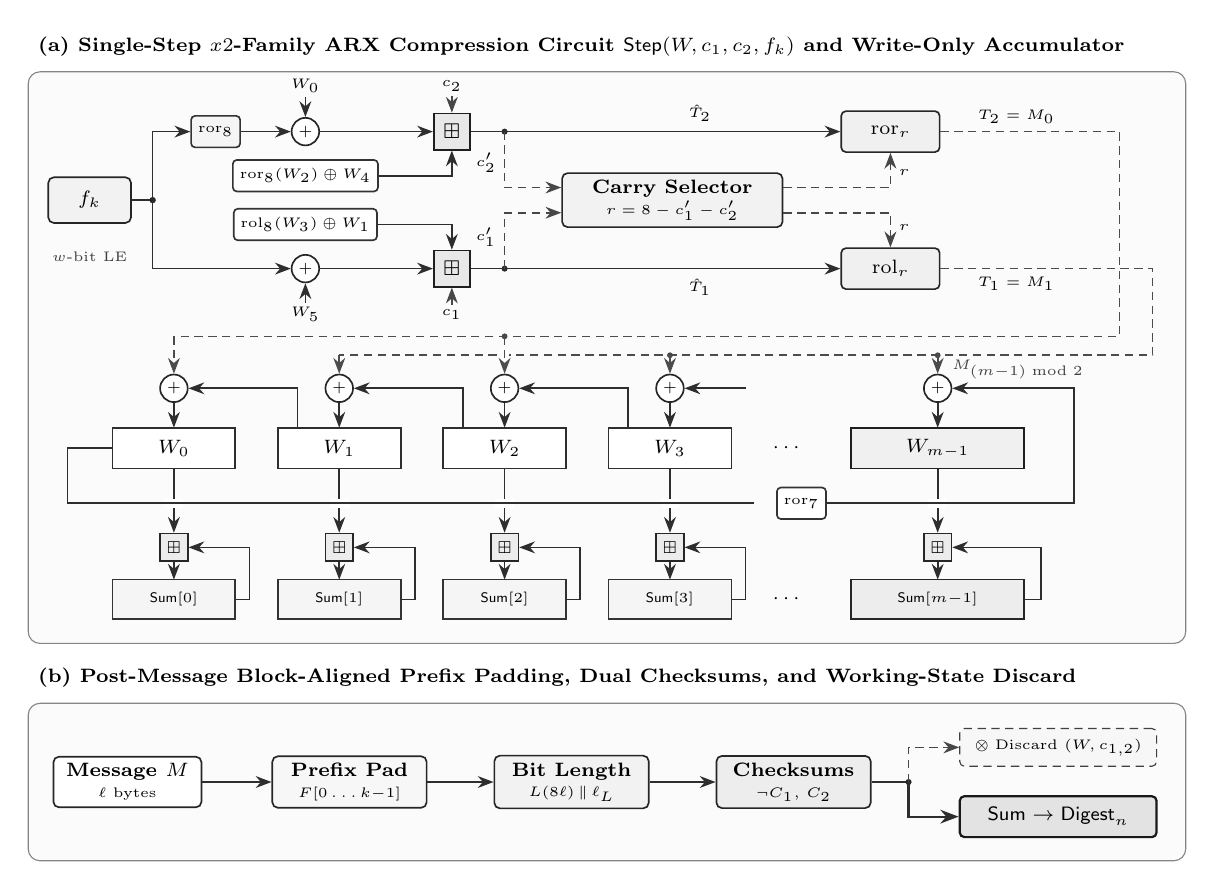
\begin{tikzpicture}[
    >=Stealth,
    xor/.style={circle, draw=black!85, semithick, fill=white, minimum size=3.5mm, inner sep=0pt, font=\tiny},
    addg/.style={rectangle, draw=black!88, semithick, fill=gray!18, minimum size=4.6mm, inner sep=0pt, font=\scriptsize\bfseries},
    sadd/.style={rectangle, draw=black!85, semithick, fill=gray!15, minimum size=3.5mm, inner sep=0pt, font=\tiny\bfseries},
    rbadge/.style={rectangle, draw=black!80, semithick, rounded corners=0.5mm, fill=gray!8, minimum height=4.0mm, inner xsep=2.5pt, inner ysep=1pt, font=\tiny},
    vrot/.style={rectangle, draw=black!85, semithick, rounded corners=0.6mm, fill=gray!12, minimum width=12.5mm, minimum height=5.2mm, inner sep=2pt, font=\scriptsize\bfseries},
    opbox/.style={rectangle, draw=black!85, semithick, rounded corners=0.7mm, fill=white, minimum height=5.8mm, inner sep=2.5pt, font=\scriptsize},
    wire/.style={->, semithick, draw=black!82},
    linew/.style={semithick, draw=black!82},
    dwire/.style={->, semithick, densely dashed, draw=black!72},
    dline/.style={semithick, densely dashed, draw=black!70},
    lbl/.style={font=\scriptsize, inner sep=1.5pt},
    tlbl/.style={font=\tiny, inner sep=1.3pt}
]

% ================= PANEL (a): SINGLE-STEP CRYPTOGRAPHIC CIRCUIT =================
\node[font=\scriptsize\bfseries, anchor=west] at (0.00, 6.22) {(a) Single-Step $x2$-Family ARX Compression Circuit $\mathsf{Step}(W, c_1, c_2, f_k)$ and Write-Only Accumulator};

\begin{scope}[on background layer]
    \draw[rounded corners=1.5mm, draw=black!48, fill=gray!3] (0.00, -1.36) rectangle (14.70, 5.90);
\end{scope}

% Upper Section: Dual Carry-Coupled ARX Mask Generator
\node[opbox, fill=gray!10, minimum width=10.5mm, font=\scriptsize\bfseries] (fk) at (0.78, 4.27) {$f_k$};
\node[tlbl, align=center, text=black!75] at (0.78, 3.55) {$w$-bit LE};

% Split from f_k
\draw[linew] (fk.east) -- (1.58, 4.27);
\fill[black!85] (1.58, 4.27) circle (1.15pt);

% Upper Mask Rail (y = 5.14): Adder 2 -> T_2
\node[rbadge] (rb_u) at (2.38, 5.14) {$\ror_8$};
\node[xor]    (xu)   at (3.52, 5.14) {$+$};
\node[rbadge, fill=white] (tap_u2) at (3.52, 4.58) {$\ror_8(W_2) \oplus W_4$};
\node[addg]   (add2) at (5.38, 5.14) {$\boxplus$};

\draw[wire] (1.58, 4.27) |- (rb_u.west);
\draw[wire] (rb_u.east) -- (xu.west);
\node[tlbl, inner sep=1.5pt] (w0tap) at (3.52, 5.72) {$W_0$};
\draw[wire] (w0tap.south) -- (xu.north);
\draw[wire] (xu.east) -- (add2.west);
\draw[wire] (tap_u2.east) -| (add2.south);
\node[tlbl, inner sep=1.5pt] (c2in) at (5.38, 5.72) {$c_2$};
\draw[dwire] (c2in.south) -- (add2.north);

% Lower Mask Rail (y = 3.40): Adder 1 -> T_1
\node[xor]    (xl)   at (3.52, 3.40) {$+$};
\node[rbadge, fill=white] (tap_l2) at (3.52, 3.96) {$\rol_8(W_3) \oplus W_1$};
\node[addg]   (add1) at (5.38, 3.40) {$\boxplus$};

\draw[wire] (1.58, 4.27) |- (xl.west);
\node[tlbl, inner sep=1.5pt] (w5tap) at (3.52, 2.82) {$W_5$};
\draw[wire] (w5tap.north) -- (xl.south);
\draw[wire] (xl.east) -- (add1.west);
\draw[wire] (tap_l2.east) -| (add1.north);
\node[tlbl, inner sep=1.5pt] (c1in) at (5.38, 2.82) {$c_1$};
\draw[dwire] (c1in.north) -- (add1.south);

% Carry Selector & Variable Rotations
\node[opbox, draw=black!85, fill=gray!10, minimum width=28.0mm, minimum height=6.4mm, align=center] (ctrl) at (8.18, 4.27)
    {\textbf{Carry Selector}\\[-0.5pt]{\tiny $r = 8 - c'_1 - c'_2$}};
\node[vrot] (rot2) at (10.95, 5.14) {$\ror_r$};
\node[vrot] (rot1) at (10.95, 3.40) {$\rol_r$};

\draw[wire] (add2.east) -- node[tlbl, above=2pt, pos=0.62] {$\hat{T}_2$} (rot2.west);
\draw[wire] (add1.east) -- node[tlbl, below=2pt, pos=0.62] {$\hat{T}_1$} (rot1.west);

\fill[black!82] (6.05, 5.14) circle (1.1pt);
\fill[black!82] (6.05, 3.40) circle (1.1pt);
\draw[dwire] (6.05, 5.14) |- node[tlbl, left=1.5pt, pos=0.28] {$c'_2$} ($(ctrl.west)+(0, 0.16)$);
\draw[dwire] (6.05, 3.40) |- node[tlbl, left=1.5pt, pos=0.28] {$c'_1$} ($(ctrl.west)+(0,-0.16)$);
\draw[dwire] ($(ctrl.east)+(0, 0.16)$) -| node[tlbl, right=1.5pt, pos=0.72] {$r$} (rot2.south);
\draw[dwire] ($(ctrl.east)+(0,-0.16)$) -| node[tlbl, right=1.5pt, pos=0.72] {$r$} (rot1.north);

% Middle Section: Cyclic Shift Register W[0..m-1] & Mask XOR Gates
\draw[dline] (rot2.east) -- (13.86, 5.14) -- (13.86, 2.54) -- (1.85, 2.54);
\node[tlbl, above=1.5pt] at (12.55, 5.14) {$T_2 = M_0$};
\draw[dline] (rot1.east) -- (14.28, 3.40) -- (14.28, 2.30) -- (3.95, 2.30);
\node[tlbl, below=1.5pt] at (12.55, 3.40) {$T_1 = M_1$};

% XOR gates above register slots at y = 1.88
\node[xor] (xw0) at (1.85, 1.88) {$+$};
\node[xor] (xw1) at (3.95, 1.88) {$+$};
\node[xor] (xw2) at (6.05, 1.88) {$+$};
\node[xor] (xw3) at (8.15, 1.88) {$+$};
\node[xor] (xwm) at (11.55, 1.88) {$+$};

\draw[->, semithick, densely dashed, draw=black!70] (1.85, 2.54) -- (xw0.north);
\fill[black!72] (6.05, 2.54) circle (1.05pt);
\draw[white, line width=3.2pt] (6.05, 2.38) -- (6.05, 2.22);
\draw[->, semithick, densely dashed, draw=black!70] (6.05, 2.54) -- (xw2.north);

\draw[->, semithick, densely dashed, draw=black!70] (3.95, 2.30) -- (xw1.north);
\fill[black!72] (8.15, 2.30) circle (1.05pt);
\draw[->, semithick, densely dashed, draw=black!70] (8.15, 2.30) -- (xw3.north);
\fill[black!72] (11.55, 2.30) circle (1.05pt);
\draw[->, semithick, densely dashed, draw=black!70] (11.55, 2.30) -- (xwm.north);
\node[tlbl, anchor=west, text=black!75] at (11.68, 2.12) {$M_{(m-1)\bmod 2}$};

% Register cells W_0, W_1, W_2, W_3, ..., W_{m-1} at y = 1.12 (0.86..1.38)
\foreach \xc/\lab/\shd in {1.85/{W_0}/white, 3.95/{W_1}/white, 6.05/{W_2}/white, 8.15/{W_3}/white} {
    \draw[semithick, draw=black!82, fill=\shd] ({\xc-0.78}, 0.86) rectangle ({\xc+0.78}, 1.38);
    \node[lbl] at (\xc, 1.12) {$\lab$};
}
\node[lbl] at (9.65, 1.12) {$\cdots$};
\draw[semithick, draw=black!88, fill=gray!12] (10.45, 0.86) rectangle (12.65, 1.38);
\node[lbl] at (11.55, 1.12) {$W_{m-1}$};

% Write arrows from XOR gates into register cells
\draw[wire] (xw0.south) -- (1.85, 1.38);
\draw[wire] (xw1.south) -- (3.95, 1.38);
\draw[wire] (xw2.south) -- (6.05, 1.38);
\draw[wire] (xw3.south) -- (8.15, 1.38);
\draw[wire] (xwm.south) -- (11.55, 1.38);

% Leftward cyclic shift wires W_{i+1} -> xw_i.east
\draw[wire] (3.42, 1.38) -- (3.42, 1.88) -- (xw0.east);
\draw[wire] (5.52, 1.38) -- (5.52, 1.88) -- (xw1.east);
\draw[wire] (7.62, 1.38) -- (7.62, 1.88) -- (xw2.east);
\draw[wire] (9.12, 1.88) -- (xw3.east);

% Modular addition gates \boxplus at y = -0.14 and Sum[0..m-1] cells at y = -0.80 (-1.05..-0.55)
\foreach \xc/\idx in {1.85/0, 3.95/1, 6.05/2, 8.15/3} {
    \node[sadd] (sa\idx) at (\xc, -0.14) {$\boxplus$};
    \draw[wire] (\xc, 0.86) -- (sa\idx.north);
    \draw[semithick, draw=black!80, fill=gray!8] ({\xc-0.78}, -1.05) rectangle ({\xc+0.78}, -0.55);
    \node[tlbl, font=\tiny\bfseries] at (\xc, -0.80) {$\SumAcc[\idx]$};
    \draw[wire] (sa\idx.south) -- (\xc, -0.55);
    \draw[wire] ({\xc+0.78}, -0.80) -- ({\xc+0.96}, -0.80) |- (sa\idx.east);
}
\node[lbl] at (9.65, -0.80) {$\cdots$};
\node[sadd] (sam) at (11.55, -0.14) {$\boxplus$};
\draw[wire] (11.55, 0.86) -- (sam.north);
\draw[semithick, draw=black!85, fill=gray!14] (10.45, -1.05) rectangle (12.65, -0.55);
\node[tlbl, font=\tiny\bfseries] at (11.55, -0.80) {$\SumAcc[m{-}1]$};
\draw[wire] (sam.south) -- (11.55, -0.55);
\draw[wire] (12.65, -0.80) -- (12.86, -0.80) |- (sam.east);

% Cyclic wrap-around W_0 -> ror_7 -> xwm.east routed cleanly along y = 0.42 with white-halo bridges
\foreach \xc in {1.85, 3.95, 6.05, 8.15, 11.55} {
    \draw[white, line width=3.4pt] ({\xc-0.12}, 0.42) -- ({\xc+0.12}, 0.42);
}
\draw[linew] (1.07, 1.12) -- (0.50, 1.12) -- (0.50, 0.42) -- (9.22, 0.42);
\node[rbadge, fill=white] (rb_wrap) at (9.82, 0.42) {$\ror_7$};
\draw[wire] (rb_wrap.east) -- (13.28, 0.42) -- (13.28, 1.88) -- (xwm.east);

% ================= PANEL (b): FINALIZATION PIPELINE & TRUNK DISCARD =================
\begin{scope}[yshift=-3.36cm]
    \node[font=\scriptsize\bfseries, anchor=west] at (0.00, 1.56) {(b) Post-Message Block-Aligned Prefix Padding, Dual Checksums, and Working-State Discard};

    \begin{scope}[on background layer]
        \draw[rounded corners=1.5mm, draw=black!48, fill=gray!3] (0.00, -0.76) rectangle (14.70, 1.24);
    \end{scope}

    \node[opbox, fill=white, minimum width=18.8mm, align=center] (p1) at (1.26, 0.24) {\textbf{Message $M$}\\[-0.5pt]{\tiny $\ell$~bytes}};
    \node[opbox, fill=gray!6, minimum width=19.6mm, align=center] (p2) at (4.08, 0.24) {\textbf{Prefix Pad}\\[-0.5pt]{\tiny $F[0\dots k{-}1]$}};
    \node[opbox, fill=gray!10, minimum width=19.6mm, align=center] (p3) at (6.90, 0.24) {\textbf{Bit Length}\\[-0.5pt]{\tiny $L(8\ell) \,\|\, \ell_L$}};
    \node[opbox, fill=gray!14, minimum width=19.6mm, align=center] (p4) at (9.72, 0.24) {\textbf{Checksums}\\[-0.5pt]{\tiny $\neg C_1,\, C_2$}};

    % Explicit split: upper branch discards (W, c1, c2); lower branch outputs Sum
    \node[rectangle, draw=black!75, densely dashed, rounded corners=0.6mm, fill=gray!6, minimum width=25.0mm, minimum height=4.8mm, inner sep=1.5pt, font=\tiny] (disc) at (13.08, 0.68) {$\otimes\;\text{Discard }(W, c_{1,2})$};
    \node[rectangle, draw=black!90, thick, rounded corners=0.6mm, fill=gray!22, minimum width=25.0mm, minimum height=5.2mm, inner sep=1.5pt, font=\scriptsize\bfseries] (dig) at (13.08, -0.20) {$\SumAcc \to \mathsf{Digest}_n$};

    \draw[wire] (p1.east) -- (p2.west);
    \draw[wire] (p2.east) -- (p3.west);
    \draw[wire] (p3.east) -- (p4.west);
    \draw[semithick, draw=black!82] (p4.east) -- (11.18, 0.24);
    \fill[black!85] (11.18, 0.24) circle (1.1pt);
    \draw[dwire] (11.18, 0.24) |- (disc.west);
    \draw[wire, thick] (11.18, 0.24) |- (dig.west);
\end{scope}

\end{tikzpicture}
\caption{Cryptographic circuit of the $x2$-family Blender hash function ($m \in \{6,7,8\}$, $t = 2$, where $M_{(m-1)\bmod 2}$ is $T_1$ for even $m$ and $T_2$ for odd $m$). \textbf{(a)}~Each step updates $(W, c_1, c_2)$ via two carry-coupled modular additions and accumulates $W'_i$ into $\SumAcc[i] \pmod{2^w}$. \textbf{(b)}~Finalization pads with $k$ cyclic $13$-byte prefix bytes (enforcing $\ge 32$ total rounds and $16$-fragment block alignment), appends $L(8\ell) \| \ell_L$, and absorbs $\neg C_1$ and $C_2$ before discarding $(W, c_1, c_2)$ and outputting $\SumAcc$ in big-endian order.}
\label{fig:blender-arch}
\end{figure}

\section{Subspace Collapse and Closed-Walk Collisions}
\label{sec:route1}

Our first collision attack targets the macro-structure of the working-state transition graph. Suppose two distinct messages $M_1 \neq M_2$ of equal byte length $\ell \ge 13$ share the same $13$-byte prefix. If both messages arrive at the end of message absorption with identical working states $(W, c_1, c_2)$, identical accumulators $\SumAcc$, and identical checksums $(C_1, C_2)$, then all three finalization stages receive identical inputs and states. This guarantees an exact full-digest collision.

\subsection{Shifted Clean Subspace Collapse}
\label{subsec:clean-subspace}
On Blender-$256$, a full working state $(W, c_1, c_2)$ has $8 \times 32 + 2 = 258$ bits, placing naive cycle search at $2^{129}$ steps. Consider instead the $m - t$ \emph{stride-$t$ XOR difference variables}:
\[
    X_i \coloneqq W_i \oplus W_{i+t} \in \{0,1\}^w, \qquad 0 \le i \le m - t - 1.
\]
Because indices $i$ and $i + t$ receive the exact same mask $M_{i \bmod t}$ in~\eqref{eq:word-shift}, the non-linear ARX masks cancel identically across the first $m - t - 1$ difference coordinates for every fragment $f_k$:
\begin{equation}
    X'_i = (W_{i+1} \oplus M_{i \bmod t}) \oplus (W_{i+t+1} \oplus M_{i \bmod t}) = X_{i+1} \qquad (0 \le i \le m - t - 2).
    \label{eq:chain-shift}
\end{equation}
Meanwhile, the boundary coordinate $i = m - t - 1$ satisfies
\begin{equation}
    X'_{m-t-1} = W_{m-t} \oplus \ror_7(W_0) \oplus M_{(m-t-1) \bmod t} \oplus M_{(m-1) \bmod t}
                = W_{m-t} \oplus \ror_7(W_0).
    \label{eq:chain-boundary}
\end{equation}
Now write $m = q t + \rho$ with $0 \le \rho < t$. Iterating $W_j = W_{j+t} \oplus X_j$ from $j = 0$ in steps of $t$ yields $W_{qt} = W_0 \oplus \bigoplus_{j=0}^{q-1} X_{jt}$. Comparing $qt$ with $m - t = (q - 1)t + \rho$ gives our first general structural theorem.

\begin{theorem}[Shifted Clean Subspace Divisibility Criterion]
\label{thm:divisibility}
Fix any constant word $x \in \{0,1\}^w$, and say that a step is \emph{$x$-clean} if the absorbed fragment $f_k$ steers $W'_0 \in \{x, \neg x\}$. Once $W_0 \in \{x, \neg x\}$, the self-XOR quantity
\begin{equation}
    \kappa(x) \coloneqq W_0 \oplus \ror_7(W_0) = x \oplus \ror_7(x)
    \label{eq:kappa-const}
\end{equation}
is invariant across both choices $W_0 = x$ and $W_0 = \neg x$ because $\neg x \oplus \ror_7(\neg x) = (x \oplus \mathbf{1}) \oplus \ror_7(x) \oplus \mathbf{1} = x \oplus \ror_7(x)$. Under consecutive $x$-clean transitions, two regimes arise:
\begin{enumerate}[leftmargin=2em]
    \item \textbf{Exact Collapse when $t \mid m$ ($\rho = 0$):} Here $m - t = (q - 1)t$, so $W_{m-t} = W_0 \oplus \bigoplus_{j=0}^{q-2} X_{jt}$. Equation~\eqref{eq:chain-boundary} then closes into the purely affine, message-independent recurrence
    \begin{equation}
        X'_i = X_{i+1} \;\;(0 \le i \le m - t - 2), \qquad
        X'_{m-t-1} = \kappa(x) \oplus \bigoplus_{j=0}^{q-2} X_{jt}.
        \label{eq:closed-chain}
    \end{equation}
    Over $\Ftwo[Z]$, the linear companion operator of~\eqref{eq:closed-chain} has characteristic polynomial $(Z^m + 1)/(Z^t + 1)$, which divides $Z^m + 1$. Thus, the trajectory of $X^{(r)}$ is strictly periodic with period dividing $m$ ($P = 8$ for $m = 8, t = 2$; $P = 6$ for $m = 6, t = 2$; $P = 9$ for $m = 9, t = 3$). At each phase $\phi \in \mathbb{Z}_P$, this collapses the $(mw + t)$-bit working state to an invariant manifold $\mathcal{C}_x^{(\phi)}$ of dimension
    \[
        \dim_{\mathrm{bits}}\bigl(\mathcal{C}_x^{(\phi)}\bigr) = 1 + (t - 1)w + t \quad \text{bits},
    \]
    parameterized solely by the complement bit $e \in \{0,1\}$ ($W_0 = x \oplus e\mathbf{1}$), the unconstrained base lanes $(W_1, \dots, W_{t-1}) \in (\{0,1\}^w)^{t-1}$, and the $t$ carry bits.
    \item \textbf{Obstruction when $t \nmid m$ ($\rho \neq 0$):} Here $m - t \equiv \rho \not\equiv 0 \pmod t$, so $W_{m-t} = W_\rho \oplus \bigoplus_{j=0}^{q-2} X_{\rho + jt}$. This injects the unconstrained lane $W_\rho$ ($\rho \in \{1, \dots, t-1\}$) into $X'_{m-t-1}$ at every step and prevents message-independent subspace closure.
\end{enumerate}
\end{theorem}

\begin{proof}
Equations~\eqref{eq:chain-shift}--\eqref{eq:closed-chain} follow directly by substituting $W_{m-t} = W_0 \oplus \bigoplus_{j=0}^{q-2} X_{jt}$ when $\rho = 0$, where $W_0 \oplus \ror_7(W_0) = \kappa(x)$ by~\eqref{eq:kappa-const}. Let $\mathcal{A}$ denote the $(m-t) \times (m-t)$ companion matrix of~\eqref{eq:closed-chain}, and let $\mathbf{e}_{m-t-1}$ denote the final standard basis vector. Applying $\mathcal{A}$ to standard basis polynomials yields the characteristic polynomial $1 + Z^t + Z^{2t} + \dots + Z^{(q-1)t} = (Z^{qt} + 1)/(Z^t + 1) = (Z^m + 1)/(Z^t + 1)$ over $\Ftwo$, so $\mathcal{A}^m = I$. Summing the affine offset $\kappa(x)$ around one $m$-step cycle contributes $(1 + \mathcal{A} + \dots + \mathcal{A}^{m-1})\mathbf{e}_{m-t-1}\,\kappa(x) = 0$ over $\Ftwo$ whenever $q = m/t$ is even ($m=8, t=2$). The same sum also vanishes via period-$6$ cancellation on $m=6, t=2$, since $(Z^6+1)/(Z^2+1) = Z^4 + Z^2 + 1$ divides $Z^6 + 1$ and $1 + \mathcal{A} + \dots + \mathcal{A}^5 = 0$. Once $X^{(r)}$ is fixed by phase $\phi = r \bmod P$, every $W_i$ ($0 \le i < m$) is uniquely reconstructed as $W_i = W_{i \bmod t} \oplus D_i^{(\phi)}$, where $D_i^{(\phi)}$ is a deterministic XOR sum of components of $X^{(\phi)}$. This leaves $1$ bit for $W_0 \in \{x, \neg x\}$, $(t-1)w$ bits for $(W_1, \dots, W_{t-1})$, and $t$ bits for the carries. When $\rho \neq 0$ (such as $m=7, t=2$ in Blender-$224$, and $m=10, t=3$), $W_\rho$ varies freely with $M_\rho$ at every step, so $X'_{m-t-1}$ depends on all subsequent message fragments.
\end{proof}

Across the $15$ parameterizations in Bradbury's specification, Theorem~\ref{thm:divisibility} partitions the family into $9$ collapsible instances ($n \in \{96, 128, 144, 192, 256, 288, 384, 512, 576\}$) and $6$ obstructed instances ($n \in \{112, 160, 224, 320, 448, 640\}$). In particular, for Blender-$256$ ($w=32, m=8, t=2$), each phase $\phi \in \mathbb{Z}_8$ has $1 + 32 + 2 = 35$ free bits. The full $8$-phase invariant clean graph $\mathcal{C}_x = \bigsqcup_{\phi=0}^{7} \mathcal{C}_x^{(\phi)}$ therefore contains $8 \times 2^{35} = 2^{38}$ states, compared to $2^{258}$ unrestricted states (a $2^{220}$-fold reduction). Similarly, Blender-$384$ ($m=6, P=6$) and Blender-$512$ ($m=8, P=8$) collapse from $386$ and $514$ bits to $6 \times 2^{67} = 2^{69.58}$ and $8 \times 2^{67} = 2^{70}$ clean states, respectively. On Blender-$512$, the subspace can be reduced further to $2 \times 2^{67} = 2^{68}$ states by first steering $X$ into its period-$2$ eigenspace $\ker(Z^2 + 1)$.

\subsection{The Parity Obstruction Theorem}
\label{subsec:parity-obstruction}
Whereas Kl\'{i}ma~\cite{Kli09} zeroed only one mask per step ($T_2 = 0$ then $T_1 = 0$, leaving a $130$-bit state across $256$-round macro-steps), Theorem~\ref{thm:divisibility} locks all six differences $X_0, \dots, X_5$ at every step ($2^{38}$ states). One might ask whether the remaining phase factor $P = 8$ on Blender-$256$ can be eliminated by steering the state into the unshifted zero-chain fixed point $X = (0,0,0,0,0,0)$, where $W_0 = W_2 = W_4 = W_6$ and $W_1 = W_3 = W_5 = W_7$. Such a fixed point would cut the subspace by another factor of $8$ to $2^{35}$ states. However, this fixed point is mathematically unreachable from the standard Blender-$256$ IV for any message sequence, even using unrestricted message words.

\begin{theorem}[Word-Parity Obstruction on Blender-$256$]
\label{thm:parity-obstruction}
For any state $W \in (\{0,1\}^{32})^8$, define the $6$-bit chain-parity vector $p(W) \coloneqq (\parop(X_0), \dots, \parop(X_5)) \in \Ftwo^6$, where $X_i = W_i \oplus W_{i+2}$. Under arbitrary message fragments $f_k \in \{0,1\}^{32}$ and arbitrary carries $(c_1, c_2)$, the following properties hold:
\begin{enumerate}[leftmargin=2em]
    \item The parity vector $p(W') = \Phi\,p(W)$ evolves strictly linearly and independently of the message, where $\Phi(p_0, p_1, p_2, p_3, p_4, p_5) = (p_1, p_2, p_3, p_4, p_5, p_0 \oplus p_2 \oplus p_4)$.
    \item On the standard Blender-$256$ initial state $W^{\mathrm{IV}}$, we have $p(W^{\mathrm{IV}}) = (1, 0, 1, 0, 0, 1) \neq \mathbf{0}$. Its orbit $\{\Phi^r p(W^{\mathrm{IV}})\}_{r \ge 0}$ consists of $8$ pairwise-distinct non-zero vectors in $\Ftwo^6$ satisfying the permanent invariants $p_4 = p_0 \oplus 1$ and $p_5 = p_1 \oplus 1$ at every step $r \ge 0$.
\end{enumerate}
Therefore, no message of any length can reach $X = \mathbf{0}$ (or even $W_0 = W_2 = W_4 = W_6$) from $W^{\mathrm{IV}}$, and the minimal clean-subspace period from $W^{\mathrm{IV}}$ is strictly $P = 8$.
\end{theorem}

\begin{proof}
Since cyclic rotation permutes bit positions, $\parop(\ror_7(W_0)) = \parop(W_0)$. Thus $\parop(W_0 \oplus \ror_7(W_0)) = \parop(W_0) \oplus \parop(\ror_7(W_0)) = 0$ holds identically for every $W_0 \in \{0,1\}^{32}$ without assuming $W_0 \in \{x, \neg x\}$. Applying $\parop(\cdot)$ to~\eqref{eq:chain-shift} and~\eqref{eq:chain-boundary} for $m=8, t=2$ gives $\parop(X'_i) = \parop(X_{i+1})$ for $0 \le i \le 4$, and
\[
    \parop(X'_5) = \parop\bigl(W_6 \oplus \ror_7(W_0)\bigr)
                 = \parop\bigl(W_0 \oplus X_0 \oplus X_2 \oplus X_4 \oplus \ror_7(W_0)\bigr)
                 = p_0 \oplus p_2 \oplus p_4.
\]
From the initial state $W^{\mathrm{IV}}$ of Blender-$256$, direct bit-popcount modulo~$2$ gives $\parop(W^{\mathrm{IV}}_{0..7}) = (0, 1, 1, 1, 0, 1, 0, 0)$, whence $p(W^{\mathrm{IV}}) = (1, 0, 1, 0, 0, 1)$. For any vector $p \in \Ftwo^6$ satisfying $p_4 = p_0 \oplus 1$ and $p_5 = p_1 \oplus 1$, its image $p' = \Phi(p)$ satisfies $p'_4 = p_5 = p_1 \oplus 1 = p'_0 \oplus 1$. Similarly, the last coordinate satisfies $p'_5 = p_0 \oplus p_2 \oplus p_4 = p_0 \oplus p_2 \oplus (p_0 \oplus 1) = p_2 \oplus 1 = p'_1 \oplus 1$. Because $p(W^{\mathrm{IV}})$ satisfies $(p_4, p_5) = (0, 1) = (p_0 \oplus 1, p_1 \oplus 1)$, induction guarantees $(p_4, p_5) = (p_0 \oplus 1, p_1 \oplus 1)$ at every step $r \ge 0$. This invariant excludes $(0,0,0,0,0,0)$ because $(p_0, p_1) = (0, 0)$ forces $(p_4, p_5) = (1, 1)$. Iterating $\Phi$ produces the $8$-cycle $(1,0,1,0,0,1) \to (0,1,0,0,1,0) \to (1,0,0,1,0,1) \to (0,0,1,0,1,1) \to (0,1,0,1,1,0) \to (1,0,1,1,0,1) \to (0,1,1,0,1,0) \to (1,1,0,1,0,0) \to (1,0,1,0,0,1)$ of $8$ distinct non-zero vectors.
\end{proof}

\subsection{Supercritical Out-Degree and Overlapping Cycle Swap}
\label{subsec:cycle-swap}
Having established that $\mathcal{C}_x$ has period $P = 8$ and size $2^{38}$ on Blender-$256$, we count the number $\deg^+(s)$ of valid $x$-clean outgoing edges leaving a state $s = (W, c_1, c_2) \in \mathcal{C}_x$. To achieve $W'_0 = W_1 \oplus T_2 = y$ for a target $y \in \{x, \neg x\}$, we require $T_2 = W_1 \oplus y$. Since $T_2 = \ror_r(\hat{T}_2)$ depends on the post-addition rotation $r \in \{6, 7, 8\}$, there are three candidate unrotated sums $\hat{T}_2^{(r)} = \rol_r(W_1 \oplus y)$ for $r \in \{6,7,8\}$. Defining $K_2 = \ror_8(W_2) \oplus W_4$,~\eqref{eq:s2} uniquely determines a candidate message fragment for each pair $(y, r) \in \{x, \neg x\} \times \{6, 7, 8\}$:
\[
    f^{(y, r)} = \rol_8\!\Bigl(\bigl((\rol_r(W_1 \oplus y) - K_2 - c_2) \bmod 2^w\bigr) \oplus W_0\Bigr).
\]
Candidate $f^{(y, r)}$ is valid if and only if running $\mathsf{Step}(W, c_1, c_2, f^{(y, r)})$ produces carry pair $(c'_1, c'_2)$ whose selected rotation $8 - (c'_1 + c'_2)$ equals the guessed $r$.

\begin{proposition}[Exact Supercritical Mean Out-Degree]
\label{prop:outdegree}
For uniformly distributed clean states in $\mathcal{C}_x$ (with $w \ge 16$), the expected number of valid $x$-clean outgoing transitions across $(y, r) \in \{x, \neg x\} \times \{6, 7, 8\}$ is
\[
    \mathbb{E}[\deg^+(s)] = 2 \times \left(\frac{1}{4} + \frac{1}{2} + \frac{1}{4}\right) = 2.000\,(1 + O(2^{-w})).
\]
If at most one valid rotation $r$ is retained per target $y \in \{x, \neg x\}$, the resulting binary-branching subgraph has mean out-degree $1.57\text{--}1.61 > 1$ (supercritical). Conversely, restricting carries to $c_1 = c_2 = 0$ ($r = 8$ only) collapses the mean out-degree below $0.64 < 1$, causing search trees to die out within $O(1)$ steps.
\end{proposition}

\begin{proof}
Fix $y \in \{x, \neg x\}$ and $r \in \{6, 7, 8\}$. In~\eqref{eq:s2}, $\alpha_2 = \ror_8(f^{(y,r)}) \oplus W_0 = (\hat{T}_2^{(r)} - K_2 - c_2) \bmod 2^w$. For uniform $(W_1, c_1, c_2)$, $\hat{T}_2^{(r)}$ and $K_2$ behave as independent uniform $w$-bit integers. When $c_2 = 0$, $c'_2 = \mathbf{1}[\hat{T}_2^{(r)} < K_2]$ has mean $(2^w - 1)/(2 \cdot 2^w) = \frac{1}{2} - 2^{-w-1}$. When $c_2 = 1$, $c'_2 = \mathbf{1}[\hat{T}_2^{(r)} \le K_2]$ has mean $\frac{1}{2} + 2^{-w-1}$. Averaging over $c_2 \in \{0,1\}$ gives $\Pr[c'_2 = 1] = \frac{1}{2}$ exactly. Meanwhile, $f^{(y,r)}$ enters adder~$1$ XORed with $W_5$ and added to $\rol_8(W_3) \oplus W_1 + c_1$, yielding $\Pr[c'_1 = 1] = \frac{1}{2} + O(2^{-w})$ independently of $c'_2$. Hence $(c'_1, c'_2)$ hits $(1,1)$ ($r=6$) with probability $\frac{1}{4}$, $(0,1)$ or $(1,0)$ ($r=7$) with probability $\frac{1}{2}$, and $(0,0)$ ($r=8$) with probability $\frac{1}{4}$. These probabilities sum to $\frac{1}{4} + \frac{1}{2} + \frac{1}{4} = 1$ per target $y \in \{x, \neg x\}$, and to $2 \times 1 = 2$ over both targets.
\end{proof}

\begin{figure}[t!]
\centering
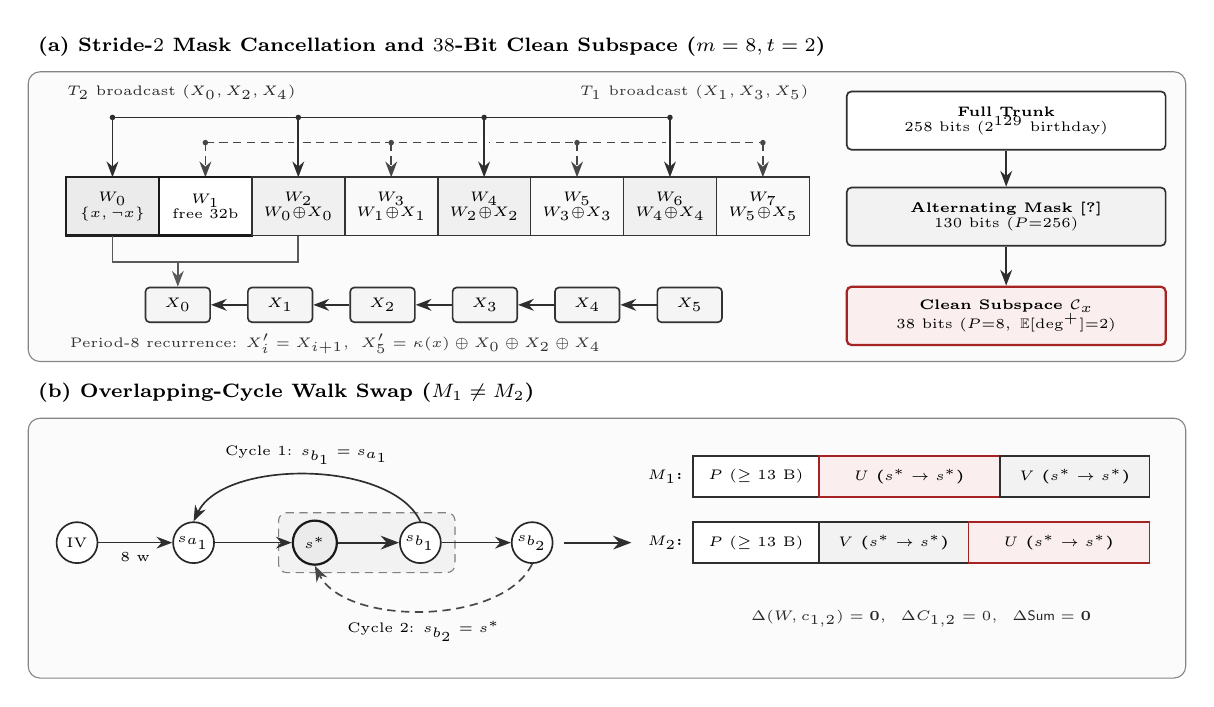
\begin{tikzpicture}[
    >=Stealth,
    snode/.style={circle, draw=black!85, semithick, fill=white, minimum size=5.2mm, inner sep=0pt, font=\tiny\bfseries},
    anode/.style={circle, draw=black!90, thick, fill=gray!16, minimum size=5.6mm, inner sep=0pt, font=\tiny\bfseries},
    xcell/.style={rectangle, draw=black!80, semithick, rounded corners=0.5mm, fill=gray!8, minimum width=8.2mm, minimum height=4.4mm, inner sep=1pt, font=\tiny\bfseries},
    scard/.style={rectangle, draw=black!82, semithick, rounded corners=0.6mm, fill=white, minimum width=38.0mm, minimum height=7.4mm, inner sep=2pt, font=\tiny, align=center},
    wire/.style={->, semithick, draw=black!82},
    dwire/.style={->, semithick, densely dashed, draw=black!72},
    lbl/.style={font=\scriptsize, inner sep=1.5pt},
    tlbl/.style={font=\tiny, inner sep=1.3pt}
]

% ================= PANEL (a): REGISTER-LANE MASK CANCELLATION & SUBSPACE COLLAPSE =================
\node[font=\scriptsize\bfseries, anchor=west] at (0.00, 5.96) {(a) Stride-$2$ Mask Cancellation and $38$-Bit Clean Subspace ($m=8, t=2$)};

\begin{scope}[on background layer]
    \draw[rounded corners=1.5mm, draw=black!48, fill=gray!3] (0.00, 1.96) rectangle (14.70, 5.64);
\end{scope}

% Mask buses above the 8-word register (T_2 solid at y=5.06, T_1 dashed at y=4.74)
\node[tlbl, anchor=west, text=black!85] at (0.44, 5.38) {$T_2$ broadcast ($X_0, X_2, X_4$)};
\node[tlbl, anchor=east, text=black!80] at (9.96, 5.38) {$T_1$ broadcast ($X_1, X_3, X_5$)};

\draw[semithick, draw=black!82] (1.07, 5.06) -- (8.15, 5.06);
\draw[semithick, densely dashed, draw=black!72] (2.25, 4.74) -- (9.33, 4.74);

\foreach \xc in {3.43, 5.79, 8.15} {
    \draw[white, line width=3.2pt] (\xc, 4.82) -- (\xc, 4.66);
}
\foreach \xc in {1.07, 3.43, 5.79, 8.15} {
    \fill[black!82] (\xc, 5.06) circle (1.0pt);
    \draw[wire] (\xc, 5.06) -- (\xc, 4.30);
}
\foreach \xc in {2.25, 4.61, 6.97, 9.33} {
    \fill[black!72] (\xc, 4.74) circle (1.0pt);
    \draw[->, semithick, densely dashed, draw=black!72] (\xc, 4.74) -- (\xc, 4.30);
}

% 8-Word Segmented Register W_0..W_7 across x = 0.48..9.92 (width 1.18cm each, y = 3.56..4.30)
\draw[thick, draw=black!88, fill=gray!16] (0.48, 3.56) rectangle (1.66, 4.30);
\node[tlbl, align=center] at (1.07, 3.93) {\textbf{$W_0$}\\[-0.5pt]$\{x, \neg x\}$};

\draw[thick, draw=black!90, fill=white] (1.66, 3.56) rectangle (2.84, 4.30);
\node[tlbl, align=center] at (2.25, 3.93) {\textbf{$W_1$}\\[-0.5pt]free $32$b};

\foreach \xL/\xc/\wlab/\xlab/\shd in {
    2.84/3.43/W_2/W_0{\oplus}X_0/gray!12,
    4.02/4.61/W_3/W_1{\oplus}X_1/gray!5,
    5.20/5.79/W_4/W_2{\oplus}X_2/gray!12,
    6.38/6.97/W_5/W_3{\oplus}X_3/gray!5,
    7.56/8.15/W_6/W_4{\oplus}X_4/gray!12,
    8.74/9.33/W_7/W_5{\oplus}X_5/gray!5
} {
    \draw[semithick, draw=black!80, fill=\shd] (\xL, 3.56) rectangle ({\xL+1.18}, 4.30);
    \node[tlbl, align=center] at (\xc, 3.93) {\textbf{$\wlab$}\\[-0.5pt]$\xlab$};
}

% Stride-2 XOR chain X_0..X_5 at y = 2.68 with message-independent shift arrows
\node[xcell] (x0) at (1.90, 2.68) {$X_0$};
\node[xcell] (x1) at (3.20, 2.68) {$X_1$};
\node[xcell] (x2) at (4.50, 2.68) {$X_2$};
\node[xcell] (x3) at (5.80, 2.68) {$X_3$};
\node[xcell] (x4) at (7.10, 2.68) {$X_4$};
\node[xcell] (x5) at (8.40, 2.68) {$X_5$};

\draw[wire] (x1.west) -- (x0.east);
\draw[wire] (x2.west) -- (x1.east);
\draw[wire] (x3.west) -- (x2.east);
\draw[wire] (x4.west) -- (x3.east);
\draw[wire] (x5.west) -- (x4.east);

% Stride-2 tap brackets from W_0, W_2 -> X_0 and boundary closure into X_5
\draw[semithick, draw=black!65] (1.07, 3.56) -- (1.07, 3.22) -- (3.43, 3.22) -- (3.43, 3.56);
\draw[wire, draw=black!65] (1.90, 3.22) -- (x0.north);
\node[tlbl, text=black!80, anchor=west] at (0.48, 2.18) {Period-$8$ recurrence: $X'_i = X_{i+1}$, \;$X'_5 = \kappa(x) \oplus X_0 \oplus X_2 \oplus X_4$};

% Right-hand State-Collapse Comparison Ladder (x = 10.36..14.48)
\node[scard, minimum width=40.5mm] (c_full) at (12.42, 5.02) {\textbf{Full Trunk}\\[-0.5pt]$258$~bits ($2^{129}$ birthday)};
\node[scard, minimum width=40.5mm, fill=gray!10] (c_kli) at (12.42, 3.80) {\textbf{Alternating Mask~\cite{Kli09}}\\[-0.5pt]$130$~bits ($P{=}256$)};
\node[scard, minimum width=40.5mm, fill=accentbg, draw=accent, thick] (c_our) at (12.42, 2.54) {\textbf{Clean Subspace $\mathcal{C}_x$}\\[-0.5pt]$38$~bits ($P{=}8,\; \mathbb{E}[\deg^+]{=}2$)};

\draw[wire] (c_full.south) -- (c_kli.north);
\draw[wire] (c_kli.south) -- (c_our.north);

% ================= PANEL (b): OVERLAPPING ANCESTOR CYCLES & COMMUTING WALK SWAP =================
\node[font=\scriptsize\bfseries, anchor=west] at (0.00, 1.56) {(b) Overlapping-Cycle Walk Swap ($M_1 \neq M_2$)};

\begin{scope}[on background layer]
    \draw[rounded corners=1.5mm, draw=black!48, fill=gray!3] (0.00, -2.06) rectangle (14.70, 1.24);
    % Shared overlap region highlight behind s* and s_{b_1}
    \draw[rounded corners=1.0mm, densely dashed, draw=black!50, fill=gray!10] (3.18, -0.72) rectangle (5.42, 0.04);
\end{scope}

% Left: Active DFS stack with two overlapping ancestor back-edges
\node[snode] (iv) at (0.62, -0.34) {$\mathrm{IV}$};
\node[snode] (a1) at (2.10, -0.34) {$s_{a_1}$};
\node[anode] (a2) at (3.64, -0.34) {$s^*$};
\node[snode] (b1) at (4.98, -0.34) {$s_{b_1}$};
\node[snode] (b2) at (6.40, -0.34) {$s_{b_2}$};

\draw[wire] (iv) -- node[tlbl, below=2pt] {$8$~w} (a1);
\draw[wire] (a1) -- (a2);
\draw[wire, thick] (a2) -- (b1);
\draw[wire] (b1) -- (b2);

\draw[wire] (b1.north) .. controls (4.60, 0.72) and (2.48, 0.72) ..
    node[tlbl, above=2pt] {Cycle $1$: $s_{b_1} = s_{a_1}$} (a1.north);
\draw[dwire] (b2.south) .. controls (6.02, -1.40) and (4.02, -1.40) ..
    node[tlbl, below=2pt] {Cycle $2$: $s_{b_2} = s^*$} (a2.south);

\draw[wire, thick] (6.80, -0.34) -- (7.66, -0.34);

% Right: Stacked Segmented Message Bars M_1 vs M_2
\node[tlbl, font=\tiny\bfseries, anchor=east] at (8.36, 0.50) {$M_1$:};
\draw[semithick, draw=black!82, fill=white]   (8.44, 0.24) rectangle (10.04, 0.76);
\draw[semithick, draw=accent, fill=accentbg]  (10.04, 0.24) rectangle (12.34, 0.76);
\draw[semithick, draw=black!82, fill=gray!10] (12.34, 0.24) rectangle (14.24, 0.76);
\node[tlbl] at (9.24, 0.50) {$P$ ($\ge 13$~B)};
\node[tlbl, font=\tiny\bfseries] at (11.19, 0.50) {$U$ ($s^* \to s^*$)};
\node[tlbl, font=\tiny\bfseries] at (13.29, 0.50) {$V$ ($s^* \to s^*$)};

\node[tlbl, font=\tiny\bfseries, anchor=east] at (8.36, -0.34) {$M_2$:};
\draw[semithick, draw=black!82, fill=white]   (8.44, -0.60) rectangle (10.04, -0.08);
\draw[semithick, draw=black!82, fill=gray!10] (10.04, -0.60) rectangle (11.94, -0.08);
\draw[semithick, draw=accent, fill=accentbg]  (11.94, -0.60) rectangle (14.24, -0.08);
\node[tlbl] at (9.24, -0.34) {$P$ ($\ge 13$~B)};
\node[tlbl, font=\tiny\bfseries] at (10.99, -0.34) {$V$ ($s^* \to s^*$)};
\node[tlbl, font=\tiny\bfseries] at (13.09, -0.34) {$U$ ($s^* \to s^*$)};

\node[tlbl, align=center, text=black!85] at (11.34, -1.30)
    {$\Delta(W, c_{1,2}) = \mathbf{0}, \;\; \Delta C_{1,2} = 0, \;\; \Delta\SumAcc = \mathbf{0}$};

\end{tikzpicture}
\caption{Shifted clean-subspace collision mechanism on Blender-$256$. \textbf{(a)}~Constraining $W'_0 \in \{x, \neg x\}$ cancels $(T_2, T_1)$ across all six stride-$2$ differences $X_0, \dots, X_5$ simultaneously, collapsing Kl\'{i}ma's $130$-bit alternating state to the $38$-bit period-$8$ clean graph $\mathcal{C}_x$. \textbf{(b)}~Re-rooting any two overlapping ancestor back-edges along a single DFS stack yields commuting closed walks $U \neq V$ at $s^*$ that collide on the full state and digest.}
\label{fig:route1-subspace}
\end{figure}

\paragraph{Single-Stage Overlapping Cycle-Swap Construction.}
Starting from $W^{\mathrm{IV}}$, $8$ deterministic greedy steps steer $W_0, W_2, W_4, W_6 \in \{x, \neg x\}$ to enter $\mathcal{C}_x$. Inside $\mathcal{C}_x$, suppose we find two distinct directed closed walks $U \neq V$ based at the same anchor state $s^* = (W^*, c_1^*, c_2^*, \phi^*) \in \mathcal{C}_x$ after a shared prefix $P$ of byte length at least $13$. Because $s^* \xrightarrow{U} s^*$ and $s^* \xrightarrow{V} s^*$ both start and end at $s^*$, three invariants hold simultaneously:
\begin{enumerate}[leftmargin=2em]
    \item Both walk lengths satisfy $|U| \equiv |V| \equiv 0 \pmod 8$. Because $(|U| + |V|) - (|V| + |U|) = 0$, the swapped messages $M_1 = P \| U \| V$ and $M_2 = P \| V \| U$ have identical byte length, identical $13$-byte prefix, and identical $16$-fragment block alignment.
    \item Every word of $U$ and $V$ appears once in $M_1$ and once in $M_2$, so $C_1(M_1) = C_1(M_2)$ and $C_2(M_1) = C_2(M_2)$ hold identically by commutativity of $(\Zmod{w}, +)$.
    \item Both $M_1$ and $M_2$ leave the working state at $s^*$. Meanwhile, during $U$ and $V$ the accumulator $\SumAcc$ undergoes pure modular translations $\SumAcc \mapsto \SumAcc \boxplus \Delta\SumAcc(s^*, U)$ and $\SumAcc \mapsto \SumAcc \boxplus \Delta\SumAcc(s^*, V)$ that commute over $(\Zmod{w})^m$:
    \begin{align*}
        \SumAcc(M_1) &= \SumAcc(P) \boxplus \Delta\SumAcc(s^*, U) \boxplus \Delta\SumAcc(s^*, V) \\
                     &= \SumAcc(P) \boxplus \Delta\SumAcc(s^*, V) \boxplus \Delta\SumAcc(s^*, U) = \SumAcc(M_2).
    \end{align*}
\end{enumerate}
One does not need two sequential birthday stages to make two cycles intersect at a common vertex $s^*$. Instead, we run a single DFS on $\mathcal{C}_x$ that checks whether the current vertex repeats an ancestor on the active DFS stack of depth $D$ (Figure~\ref{fig:route1-subspace}(b)). Any two ancestor back-edges $[a_1, b_1)$ ($s_{b_1} = s_{a_1}$) and $[a_2, b_2)$ ($s_{b_2} = s_{a_2}$) whose intervals overlap ($\max(a_1, a_2) < \min(b_1, b_2)$) automatically share every vertex in $[\max(a_1, a_2), \min(b_1, b_2))$. Re-rooting both cycles at $s^* = s_{\max(a_1, a_2)}$ immediately produces commuting closed walks $U \neq V$ in expected work $O(|\mathcal{C}_x|/D)$ when $D \le \sqrt{|\mathcal{C}_x|}$, or $O(\sqrt{|\mathcal{C}_x|}) = O(2^{19})$ overall. Using $8$ threads sharing a short common trunk prefix, our pure-C solver finds verified $16{,}000$-byte standard-IV Blender-$256$ collisions in $0.045$~s (fast seed) and $0.73$~s mean across $10$ cold seeds ($0.18$~s min, $1.42$~s max).

\subsection{Multicollisions and Higher-Digest Scaling}
\label{subsec:route1-scaling}
Once a single $(P, U, V)$ tuple at $s^*$ is found (in under $1$~s on Blender-$256$), we can concatenate $r$ copies of $U$ and $r$ copies of $V$ in any balanced arrangement. Each arrangement $P \| W_1 \| \dots \| W_{2r}$ chooses $W_j \in \{U, V\}$ with $\#\{j : W_j = U\} = r$. This yields $\binom{2r}{r} \approx 4^r / \sqrt{\pi r}$ pairwise-distinct messages of identical byte length that all hash to the exact same Blender-$256$ digest with zero additional search work. In our experiments, we verified all $\binom{6}{3} = 20$ colliding messages on the official C reference at $r=3$, and the same witness generates $\binom{96}{48} \approx 2^{92.4}$ colliding messages at $r = 48$.

For the $64$-bit variants Blender-$384$ ($|\mathcal{C}_x| = 6 \cdot 2^{67} \approx 2^{69.58}$) and Blender-$512$ ($|\mathcal{C}_x| = 8 \cdot 2^{67} = 2^{70}$, or $2^{68}$ on the period-$2$ chain eigenspace), capping the DFS path length at $\ell$ words yields overlapping ancestor cycles in $\Theta(|\mathcal{C}_x|/\ell)$ evaluations. At a practical message budget of $32$~KB ($\ell = 2^{12}$ words), this requires $2^{57.6}$ rounds on Blender-$384$ and $2^{56}\text{--}2^{58}$ rounds on Blender-$512$ with $O(\ell)$ memory. Unrestricted path lengths reach the birthday knee $\sqrt{|\mathcal{C}_x|} \approx 2^{34.8}$ and $2^{34}\text{--}2^{35}$ rounds, improving over the $2^{192}$ and $2^{256}$ birthday bounds and avoiding Kl\'{i}ma's $\ge 2^{275}$- and $2^{340}$-word wound messages~\cite{Kli09}.

\section{Silent Carry Injection and Minimal-Length Collisions}
\label{sec:route2}

Although the closed-walk subspace attack achieves sub-second collisions on Blender-$256$, it has two structural limitations. First, it requires message lengths of several thousand words to close a cycle in $\mathcal{C}_x$. Second, by Theorem~\ref{thm:divisibility}, it is algebraically obstructed on odd-word Blender-$224$ ($m=7, t=2$). We now construct a local two-step ARX differential trail that overcomes both barriers simultaneously.

\subsection{Silent Carry Injection and Complement Healing}
\label{subsec:silent-carry}
Following the local perturbation-and-correction paradigm~\cite{CJ98}, suppose two trajectories agree on the entire state $(W^{(p)}, c_1^{(p)}, c_2^{(p)}, \SumAcc^{(p)})$ entering step~$p$. They absorb two distinct word pairs $(w_p, w_{p+1}) \neq (w'_p, w'_{p+1})$ at steps~$p$ and~$p+1$, and re-merge on $(W^{(p+2)}, c_1^{(p+2)}, c_2^{(p+2)}, \SumAcc^{(p+2)})$ while preserving both modular checksums $C_1$ and $C_2$.

\paragraph{Step $p$: Silent Carry Injection.}
For distinct message words $w_p \neq w'_p$ to produce zero difference in $W^{(p+1)}$ (and hence zero difference in $\SumAcc^{(p+1)}$),~\eqref{eq:word-shift} requires $\Delta W^{(p+1)} = \mathbf{0} \iff (T'_1, T'_2) = (T_1, T_2)$. If $(c'_1, c'_2)$ remained equal across both branches, equal rotations $r' = r$ would force $\hat{T}'_1 = \hat{T}_1$, whence $w'_p = w_p$. Thus, the only viable differential transition flips both output carries between $(0, 0)$ (rotation $r = 8$) and $(1, 1)$ (rotation $r' = 6$) while compensating the $2$-bit rotation shift inside the pre-rotation modular sums. Let the state-dependent second addends at step~$p$ be
\[
    K_1 = \bigl(\rol_8(W^{(p)}_3) \oplus W^{(p)}_1\bigr) + c_1^{(p)}, \qquad
    K_2 = \bigl(\ror_8(W^{(p)}_2) \oplus W^{(p)}_4\bigr) + c_2^{(p)}.
\]
Put $x = w_p \oplus W^{(p)}_5$ and $x' = w'_p \oplus W^{(p)}_5$ in adder~$1$, and put $y = \ror_8(w_p) \oplus W^{(p)}_0$ and $y' = \ror_8(w'_p) \oplus W^{(p)}_0$ in adder~$2$, so that $x \oplus x' = \Delta_x$ and $y \oplus y' = \ror_8(\Delta_x)$. Requiring $(c^{(p+1)}_1, c^{(p+1)}_2) = (0,0)$ on branch~$M$ ($x + K_1 = u < 2^w$, $y + K_2 = v < 2^w$, $r = 8$) and $(1, 1)$ on branch~$M'$ ($x' + K_1 = 2^w + \rol_2(u)$, $y' + K_2 = 2^w + \ror_2(v)$, $r' = 6$) yields
\[
    T_1 = \rol_8(u) = \rol_6(\rol_2(u)) = T'_1, \qquad
    T_2 = \ror_8(v) = \ror_6(\ror_2(v)) = T'_2.
\]
Both $W^{(p+1)}$ and $\SumAcc^{(p+1)}$ therefore remain bit-for-bit identical across the two branches, and the entire perturbation is hidden inside the $2$-bit carry differential $(0,0) \leftrightarrow (1,1)$.

\begin{theorem}[Step-$(p+1)$ Complement Healing Rigidity]
\label{thm:healing-rigidity}
Suppose two executions enter step~$p+1$ with identical working words $W^{(p+1)}$ and opposite symmetric carry pairs $(c_1, c_2) = (0, 0)$ on branch~$M$ versus $(c'_1, c'_2) = (1, 1)$ on branch~$M'$. Step~$p+1$ achieves $\Delta W^{(p+2)} = \mathbf{0}$, $\Delta(c_1^{(p+2)}, c_2^{(p+2)}) = (0, 0)$, and $\Delta(C_1, C_2) = (0, 0)$ if and only if all three conditions hold:
\begin{enumerate}[leftmargin=2em]
    \item \textbf{Exact Bitwise-Complement Message Words:} The second-step message words satisfy $w'_{p+1} = \neg w_{p+1}$, so that $\Delta w_{p+1} = 2^w - 1$.
    \item \textbf{Mid-Point Input Locking and Register Alignment:} The active adder inputs equal $(w_{p+1} \oplus W^{(p+1)}_5,\, w'_{p+1} \oplus W^{(p+1)}_5) = (2^{w-1}, 2^{w-1} - 1)$ and $(\ror_8(w_{p+1}) \oplus W^{(p+1)}_0,\, \ror_8(w'_{p+1}) \oplus W^{(p+1)}_0) = (2^{w-1}, 2^{w-1} - 1)$. This uniquely fixes $w_{p+1} = W^{(p+1)}_5 \oplus 2^{w-1}$ and imposes the $w$-bit register alignment condition
    \begin{equation}
        W^{(p+1)}_0 = \ror_8(W^{(p+1)}_5) \oplus 2^{w-1} \oplus \ror_8(2^{w-1}),
        \label{eq:w0-w5-lock}
    \end{equation}
    which simplifies to $W^{(p+1)}_0 = \ror_8(W^{(p+1)}_5) \oplus \mathtt{0x80800000}$ when $w = 32$.
    \item \textbf{Dual Modular Checksum Cancellation:} Both $C_1$ and $C_2$ match after step~$p+1$ if and only if $(w'_p - w_p)$ is odd and the low $w - 1$ bits of $w_{p+1}$ satisfy the $(w-1)$-bit congruence
    \begin{equation}
        2\,w_{p+1} \equiv w'_p - w_p - 1 \pmod{2^w}.
        \label{eq:checksum-heal}
    \end{equation}
\end{enumerate}
\end{theorem}

\begin{proof}
Equal next carries $(c''_1, c''_2)$ across both branches force equal rotations $r'' = 8 - (c''_1 + c''_2)$. Requiring $\Delta W^{(p+2)} = \mathbf{0}$ then forces equal unrotated sums $\hat{T}''_1, \hat{T}''_2$ and equal carries $(c''_1, c''_2)$, so the exact integer sums over $\mathbb{Z}$ in both adders must match. Let $A = w_{p+1} \oplus W^{(p+1)}_5$, $A' = w'_{p+1} \oplus W^{(p+1)}_5$, $D = \ror_8(w_{p+1}) \oplus W^{(p+1)}_0$, and $D' = \ror_8(w'_{p+1}) \oplus W^{(p+1)}_0$. Integer equality against $(c_1, c_2) = (0,0)$ versus $(c'_1, c'_2) = (1,1)$ requires $A - A' = 1$ and $D - D' = 1$ over $\mathbb{Z}$, while bitwise XOR satisfies $D \oplus D' = \ror_8(A \oplus A') = \ror_8(\Delta w_{p+1})$. Subtracting $1$ from $A$ in binary flips a contiguous low-bit suffix of length $k \ge 1$ ($A \oplus A' = 2^k - 1$). For $1 \le k \le w$ and $w \ge 16$, the mask $2^k - 1$ is invariant under $\ror_8$ if and only if $k = w$. Thus $A \oplus A' = D \oplus D' = 2^w - 1$, which uniquely forces $(A, A') = (D, D') = (2^{w-1}, 2^{w-1} - 1)$. Hence $w'_{p+1} = \neg w_{p+1}$, $w_{p+1} = W^{(p+1)}_5 \oplus 2^{w-1}$, and substituting $w_{p+1}$ into $D = 2^{w-1}$ gives~\eqref{eq:w0-w5-lock}. Conversely, for any state addends $B_1, B_2 \in \{0, \dots, 2^w - 1\}$, $2^{w-1} + B_i + 0 = (2^{w-1} - 1) + B_i + 1$ holds identically over $\mathbb{Z}$, producing identical $(\hat{T}''_1, \hat{T}''_2)$ and identical $(c''_1, c''_2)$. Finally, by~\eqref{eq:checksums}, equal length reduces $\Delta(C_1, C_2) = (0,0)$ to $w_p + w_{p+1} \equiv w'_p + (2^w - 1 - w_{p+1}) \pmod{2^w}$. This rearranges to~\eqref{eq:checksum-heal}, requires $w'_p - w_p$ odd, and fixes the low $w - 1$ bits of $w_{p+1}$ and $W^{(p+1)}_5$.
\end{proof}

\subsection{Healing Probability Across Word Counts}
\label{subsec:healing-density}
Every equation in Section~\ref{subsec:silent-carry} and Theorem~\ref{thm:healing-rigidity} at steps~$p$ and~$p+1$ accesses only working words $W_0, W_1, W_2, W_3, W_4, W_5$ and carries $(c_1, c_2)$, without touching $W_6, \dots, W_{m-1}$. Therefore, the local two-step silent-carry healing mechanism applies identically to every $x2$-family variant $m \in \{6, 7, 8\}$, bypassing the $t \nmid m$ obstruction on $7$-word Blender-$224$.

We now compute the exact probability that a random reachable state $(W^{(p)}, c_1^{(p)}, c_2^{(p)})$ at $w = 32$ admits an unordered colliding pair $\{(w_p, w_{p+1}), (w'_p, w'_{p+1})\}$. In a single $32$-bit adder, $x + K_1 = u < 2^{32}$ and $x' + K_1 = 2^{32} + \rol_2(u)$ hold if and only if $d_1 = x' - x > 0$ satisfies $d_1 = 2^{32} + \rol_2(u) - u$. Writing $u = 2^{30} q + r$ ($q \in \{0,1,2,3\}$, $0 \le r < 2^{30}$) gives $\rol_2(u) - u = 3r - (2^{32} - 1)q$, so $d_1 \equiv 0 \pmod 3$. Summing exact valid ranges over $q \in \{0,1,2,3\}$ with $M = (2^{30} - 1)/3$ gives the single-adder validity ratio
\[
    \frac{N_1}{2^{64}} = \frac{21 M^2 + 9 M}{2^{64}} = 0.145833333236\dots \approx \frac{7}{48} = 2^{-2.7776}.
\]
Across both adders simultaneously (coupled by $y \oplus y' = \ror_8(x \oplus x')$), independent XOR alignment predicts $(7/48)^2 = 2^{-5.555}$ unordered silent step-$p$ pairs per state. Requiring $w'_p - w_p$ odd ($\frac{1}{2}$), the $32$-bit alignment~\eqref{eq:w0-w5-lock} ($2^{-32}$), and the $31$-bit checksum congruence~\eqref{eq:checksum-heal} ($2^{-31}$) yields the analytical prediction
\begin{equation}
    \mathbb{E}\bigl[\#\text{unordered valid healing pairs per state}\bigr]
    = \Bigl(\frac{7}{48}\Bigr)^2 \cdot 2^{-1} \cdot 2^{-32} \cdot 2^{-31} = 2^{-69.555},
    \label{eq:route2-prob}
\end{equation}
corresponding to $2^{-68.555}$ ordered transitions (since swapping $(M, M')$ and $(M', M)$ represents the same colliding pair). Across $10^7$-state parallel Monte Carlo audits using a complete $6$-step algebraic contraction cross-checked against exact bit-level DFS, we measure $2^{-69.558 \pm 0.004}$ on $7$-word Blender-$224$ and $2^{-69.579 \pm 0.005}$ on $8$-word Blender-$256$, matching~\eqref{eq:route2-prob}. Because each random reachable state yields an unordered colliding pair with probability $2^{-69.558}$, this two-step trail breaks standard-IV Blender-$224$ in $2^{69.56}$ state evaluations ($\ll 2^{112}$ birthday bound) using $24$-byte ($6$-word) messages.

\subsection{Closed-Form Semi-Free-Start Collisions}
\label{subsec:closed-form-sfs}
Before inverting from the fixed standard IV, we characterize semi-free-start (SFS) collisions, in which the attacker selects an initial working register $W^{(0)} \in (\{0,1\}^w)^m$ (keeping standard initial carries $c_1^{(0)} = c_2^{(0)} = 0$ and $\SumAcc^{(0)} = \mathbf{0}$) and distinct messages $M_1 \neq M_2$.

\paragraph{Provable $1$-Round Prefix Minimum and Prefix-Pad Truncation.}
With $p = 0$ shared prefix words, the active pair $(w_0, w_1) \neq (w'_0, w'_1)$ occupies bytes $0 \dots 2b-1$. Even $k = 1$ cyclic prefix-pad byte during finalization then replays differing message bytes without healing alignment, while $c_1^{(0)} = c_2^{(0)} = 0$ precludes borrow absorption. Instead, take $p = 1$ shared prefix word $w_0$ ($b$ bytes) followed by active words $(w_1, w_2) \neq (w'_1, w'_2)$. We pad with trailing zero bytes up to $\ell = 113$ bytes for $w = 32$ ($B_{\mathrm{blk}} = 64$, $\ell_L = 2$, $2b = 8$) or $\ell = 229$ bytes for $w = 64$ ($B_{\mathrm{blk}} = 128$, $\ell_L = 2$, $2b = 16$). The cyclic prefix-pad count then equals
\[
    k_{32} = 64 - ((113 + 2 + 8 + 1) \bmod 64) = 4~\text{B}, \qquad
    k_{64} = 128 - ((229 + 2 + 16 + 1) \bmod 128) = 8~\text{B}.
\]
Thus $k = b$ bytes exactly, so finalization replays only the single shared prefix word $w_0 = F[0 \dots b-1]$ and never touches $(w_1, w_2)$.

\begin{theorem}[Deterministic $O(1)$ Closed-Form SFS Across All Four NIST Variants]
\label{thm:sfs-all}
Fix $c_1^{(0)} = c_2^{(0)} = 0$. Across all four official NIST Blender instances (Blender-$224$, Blender-$256$, Blender-$384$, and Blender-$512$), valid SFS colliding triples $(W^{(0)}, M_1, M_2)$ of length $113$~B ($w=32$) and $229$~B ($w=64$) can be generated in deterministic $O(1)$ closed form with zero trial loops and zero retries:
\begin{enumerate}[leftmargin=2em]
    \item \textbf{Even $8$-Word Variants ($m = 8$: Blender-$256$ and Blender-$512$):} Choosing $x' = y' = 0$ and $2^w - x = 3$ fixes constant step-$1$ masks $(T_1, T_2)$ and step-$1$ state targets $W^{(1)}_0, W^{(1)}_1, W^{(1)}_3, W^{(1)}_6$ for any seed $W^{(1)}_5 \in \{0,1\}^w$. Setting prefix-round mask $t_1 = 0$ leaves $W^{(1)}_2, W^{(1)}_4, W^{(1)}_7$ unconstrained, solving the single prefix round by direct substitution.
    \item \textbf{Odd $7$-Word Variant ($m = 7$: Blender-$224$):} Because $m = 7$ lacks $W_7$ and wraps via $W^{(1)}_6 = \ror_7(W^{(0)}_0) \oplus t_2$, setting $t_1 = 0$ overconstrains the prefix round. Instead, choosing $t_1(t_2) = \rol_{16}(\rol_7(W^{(1)}_6 \oplus t_2) \oplus \ror_8(W^{(1)}_4 \oplus t_2))$ annihilates the first summand of prefix adder~$2$ ($\ror_8(w_0) \oplus W^{(0)}_0 = 0$). This eliminates all integer addition carries and reduces the remaining consistency condition to the carry-free $\Ftwo$-circulant equation
    \begin{equation}
        M_{224}(X)\,t_2(X) = R(X) \pmod{X^{32} + 1}, \qquad M_{224}(X) = X^{15}(1 + X + X^8).
        \label{eq:sfs-224}
    \end{equation}
    Since $M_{224}(1) = 3 \equiv 1 \pmod 2$ has odd weight and $(X^{32} + 1) = (X + 1)^{32}$ over $\Ftwo$, $M_{224}(X)$ is an exact bijection on $\Ftwo[X]/(X^{32} + 1)$, inverted in $5$ XOR-shift squaring steps for every $32$-bit seed $W^{(1)}_5$.
    \item \textbf{Short $6$-Word Variant ($m = 6$: Blender-$384$):} Here both $W^{(1)}_6$ and $W^{(1)}_7$ are absent ($W^{(1)}_5 = \ror_7(W^{(0)}_0) \oplus t_1$). Choosing sparse $\Delta_x = \mathtt{0x8000000000000041}$ and aligning the low byte of $W^{(1)}_5$ so $y' < 2^{55}$ decouples $\ror_8(\Delta_x)$ from $y'$ without carry interaction. Enforcing the $1$-bit parity invariant of $(1 + X^{41})$ via a deterministic borrow-preserving bit-$8$ toggle on $W^{(1)}_5$ reduces prefix inversion over $\Ftwo[X]/(X^{64} + 1)$ to a single $64$-bit carryless multiplication by the circulant inverse $L_{384}(X)^{-1} = \mathtt{0xbbbbdddeeeef7777}$.
\end{enumerate}
\end{theorem}

\begin{proof}
In all four constructions, $(w_1, w_2)$ and $(w'_1, w'_2 = \neg w_2)$ satisfy the step-$1$ silent carry equations ($u < 2^w$, $v < 2^w$ versus $2^w + \rol_2(u)$, $2^w + \ror_2(v)$) and Theorem~\ref{thm:healing-rigidity} at step~$2$ by choice of $(W^{(1)}_0, \dots, W^{(1)}_5)$. For $m = 8$, direct substitution into $\mathsf{Step}(W^{(0)}, 0, 0, w_0)$ yields $s_1 = 0$ ($c'_1 = 0$), $s_2 < 2^w$ ($c'_2 = 0$), $r = 8$, and $W^{(1)}$. For $m = 7$, annihilating $\ror_8(w_0) \oplus W^{(0)}_0 = 0$ sets prefix $s_2 = \ror_8(W^{(0)}_2) \oplus W^{(0)}_4 < 2^{32}$ ($c'_2 = 0$), and $s_1 = \rol_8(t_1) < 2^{32}$ ($c'_1 = 0$, $r = 8$). Substituting $W^{(0)}$ in terms of $(W^{(1)}, t_1, t_2)$ collapses $\hat{t}_2 = \rol_8(t_2)$ to~\eqref{eq:sfs-224}, where $M_{224}(X)^{-1} = \prod_{j=0}^{4} M_{224}(X)^{2^j} \bmod (X^{32} + 1)$ as established in Section~\ref{subsec:prelim}. For $m = 6$, we eliminate $t_1$ modulo $(1 + X^{41})$. Since $\gcd(41, 64) = 1$, $\im(1 + X^{41})$ is the codimension-$1$ even-weight hyperplane, which is matched by toggling bit~$8$ of $W^{(1)}_5$ ($y' = \cdots 10_2 \leftrightarrow \cdots 11_2$ preserves the popcount of $t - y'$). This yields an odd-weight circulant operator $L_{384}(X)$ with unique inverse $\mathtt{0xbbbbdddeeeef7777}$ in $\Ftwo[X]/(X^{64} + 1)$, after which $t_1$ is recovered uniquely along the $64$-cycle of stride $41 \bmod 64$.
\end{proof}

\subsection{Minimal-Length and Identical-Prefix Inversion}
\label{subsec:purec-inversion}
We now turn to the fixed standard SHA-$256$ initialization vector $W^{\mathrm{IV}}$ on Blender-$256$.

\begin{proposition}[Global $24$-Byte Minimum Standard-IV Collision Length]
\label{prop:24b-min}
Under the standard initialization vector $W^{\mathrm{IV}}$ of Blender-$256$, no colliding pair $M_1 \neq M_2$ of equal byte length $\ell \le 23$ exists within the two-step silent-carry healing family. A message pair consisting of $p = 4$ shared prefix words ($16$ bytes) followed by $2$ active words ($8$ bytes), totaling $\ell = 24$ bytes ($6$ words), achieves the exact global minimum length from $W^{\mathrm{IV}}$ (matching the $24$-byte length previously known only for the unreachable all-zero state~\cite{XL08}).
\end{proposition}

\begin{proof}
For $\ell < 64$~B, Stage~1 of finalization replays all $\min(\ell, 13)$ prefix bytes $F[0 \dots \min(\ell, 13)-1]$ cyclically across $k = 119 - \ell - \ell_L \ge 94$ pad bytes. Any difference inside the first $13$ bytes ($M_1[0 \dots 12] \neq M_2[0 \dots 12]$) is re-injected more than $7$ times during padding from unsynchronized working states, breaking the collision. Since fragments are $4$-byte words, $M_1$ and $M_2$ must share at least $p \ge \lceil 13 / 4 \rceil = 4$ prefix words ($16$ bytes, $w_0 \dots w_3$). They also require at least $2$ active words $(w_4, w_5) \neq (w'_4, w'_5)$ ($8$ bytes) because a $1$-word difference alters $(C_1, C_2)$ non-trivially ($w'_4 \neq w_4 \implies C_1(M_1) \neq C_1(M_2)$). In addition, if $\ell \in \{21, 22, 23\}$ is not a multiple of $4$, trailing incomplete residue bytes mix directly with $F[0]$ before healing completes. Exhaustive bit-vector unsatisfiability checks over $\ell \le 23$ confirm that $\ell = 24$ bytes ($6$ words) is minimal.
\end{proof}

\paragraph{Solver-Free $4$-Round Lane-Invariant and Byte-Lattice Inversion.}
Feeding a $4$-round ARX prefix $(w_0, w_1, w_2, w_3)$ directly to general-purpose SMT solvers fails to scale. In controlled benchmarks, Z3 times out ($> 90$~s) on $7 / 7$ unconstrained and partially constrained $4$-round instances. Adapting algebraic message modification~\cite{WY05} to Blender's carry-coupled ARX round, we eliminate SAT/SMT solvers by exploiting two algebraic decompositions of $4$ consecutive $x2$-family rounds $I \xrightarrow{w_0, w_1} S \xrightarrow{w_2, w_3} W^{(4)}$ (Figure~\ref{fig:route2-healing}):
\begin{enumerate}[leftmargin=2em]
    \item \textbf{Four-Round Parity-Lane Invariants:} Consider $4$ rounds from any starting state $I$, which is either $W^{\mathrm{IV}}$ for $24$-byte standard-IV collisions or the post-prefix state $W(P_{\mathrm{ip}})$ after an arbitrary $16$-byte shared prefix $P_{\mathrm{ip}}$ for $40$-byte identical-prefix collisions (as distinct from two-prefix chosen-prefix collisions~\cite{SLdW07}). Tracking odd and even register lanes cancels intermediate masks and yields two $8$-bit byte-XOR invariants on the step-$4$ addends $(K_1, K_2)$:
    \[
        \bigoplus_{j=0}^{3} \mathrm{byte}_j\bigl(K_1 \oplus I_5 \oplus \rol_8(I_7)\bigr) = 0, \qquad
        \bigoplus_{j=0}^{3} \mathrm{byte}_j\bigl(K_2 \oplus \ror_7(I_0) \oplus \ror_8(I_6)\bigr) = 0.
    \]
    In addition, we obtain $\im(\mathrm{id} \oplus \ror_7)$ even-popcount filters on $(W^{(4)}_5 \oplus Q \oplus I_1)$ and $(W^{(4)}_6 \oplus P \oplus I_2)$, where $\mathrm{id}$ denotes the $32$-bit identity map, $P = W^{(4)}_0 \oplus W^{(4)}_2$, and $Q = W^{(4)}_1 \oplus W^{(4)}_3$. Inverting $(\mathrm{id} \oplus \ror_7)$ along the single $32$-cycle of stride $7 \bmod 32$ ($\gcd(7, 32) = 1$) fixes $12$ exact $2$-round bridge targets $(S, e_1, e_2) \xrightarrow{w_2, w_3} (P^*, Q^*)$ per outer candidate.
    \item \textbf{Two-Round $r = 8$ Byte-Lattice Nibble Contraction ($131{,}072\times$ Speedup):} On the $r_2 = r_3 = 8$ branch ($c'_1 = c'_2 = 0$ across steps~$2$ and~$3$), let $u_a = \hat{T}_1^{(2)}$, $v_a = \hat{T}_2^{(2)}$, $u_b = \hat{T}_1^{(3)}$, and $v_b = \hat{T}_2^{(3)}$. The target conditions $\rol_8(u_a) \oplus \ror_8(v_b) = \Delta_P^*$ and $\ror_8(v_a) \oplus \rol_8(u_b) = \Delta_Q^*$ express $(u_b, v_b)$ directly in terms of $(v_a, u_a)$, while eliminating $w_3$ between step-$3$ adders couples $u_a$ and $v_a$ byte-by-byte. Splitting each byte of $w_2$ into a $6$-bit low slice $L_j$ and a $2$-bit top crumb $z_j$ ($4 \times 2 = 8$ bits across all four bytes) decouples inter-byte carries. Denoting by $\rol_2^{(4)}$ the $2$-bit cyclic crumb shift across the $8$-bit top-crumb vector $z_{\mathrm{nib}} = (z_0, z_1, z_2, z_3) \in \Ftwo^8$, we obtain the $4$-cycle linear nibble equation $z_{\mathrm{nib}} \oplus \rol_2^{(4)}(z_{\mathrm{nib}}) = R_{\mathrm{nib}}$, which reduces $256$ guesses to $4$. Meanwhile, the four $6$-bit low slices $L_j$ lie in independent intervals of width at most $16$, shrinking the search space from $2^{32}$ to $2^{15}$ operations ($131{,}072\times$ reduction, $0.11\text{--}0.29$~ms per $2$-round call in pure C).
\end{enumerate}

\begin{figure}[t!]
\centering
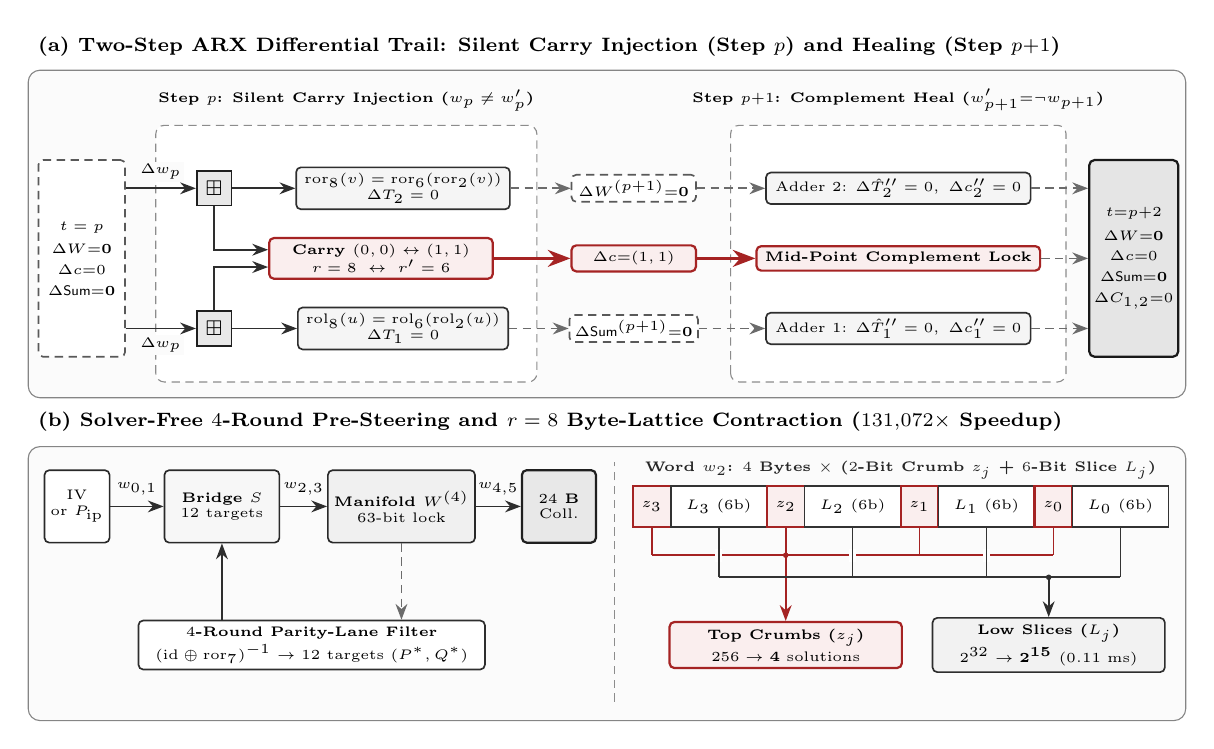
\begin{tikzpicture}[
    >=Stealth,
    addg/.style={rectangle, draw=black!88, semithick, fill=gray!18, minimum size=4.4mm, inner sep=0pt, font=\scriptsize\bfseries},
    cbox/.style={rectangle, draw=black!82, semithick, rounded corners=0.6mm, fill=white, inner xsep=3pt, inner ysep=2.2pt, font=\tiny, align=center},
    zbadge/.style={rectangle, draw=black!65, semithick, densely dashed, rounded corners=0.6mm, fill=white, inner xsep=2.5pt, inner ysep=2pt, font=\tiny, align=center},
    abadge/.style={rectangle, draw=accent, thick, rounded corners=0.6mm, fill=accentbg, inner xsep=3pt, inner ysep=2.2pt, font=\tiny\bfseries, align=center},
    pbox/.style={rectangle, draw=black!84, semithick, rounded corners=0.6mm, fill=white, minimum height=9.2mm, inner xsep=2.2pt, inner ysep=2pt, font=\tiny, align=center},
    wire/.style={->, semithick, draw=black!82},
    actwire/.style={->, line width=1.15pt, draw=accent},
    zwire/.style={->, semithick, densely dashed, draw=black!58},
    lbl/.style={font=\scriptsize, inner sep=1.5pt},
    tlbl/.style={font=\tiny, inner sep=1.3pt}
]

% ================= PANEL (a): TWO-STEP SILENT-CARRY DIFFERENTIAL TRAIL =================
\node[font=\scriptsize\bfseries, anchor=west] at (0.00, 6.24) {(a) Two-Step ARX Differential Trail: Silent Carry Injection (Step $p$) and Healing (Step $p{+}1$)};

\begin{scope}[on background layer]
    \draw[rounded corners=1.5mm, draw=black!48, fill=gray!3] (0.00, 1.78) rectangle (14.70, 5.94);
    \draw[rounded corners=1.1mm, densely dashed, draw=black!45, fill=white] (1.62, 1.98) rectangle (6.46, 5.24);
    \draw[rounded corners=1.1mm, densely dashed, draw=black!45, fill=white] (8.92, 1.98) rectangle (13.18, 5.24);
\end{scope}

% Entry checkpoint t = p
\node[zbadge, minimum width=11.0mm, minimum height=25.0mm] (st_p) at (0.68, 3.55) {\textbf{$t = p$}\\[2.5pt]$\Delta W{=}\mathbf{0}$\\[1.5pt]$\Delta c{=}0$\\[1.5pt]$\Delta\SumAcc{=}\mathbf{0}$};

% Step p Sub-panel: Silent Carry Injection
\node[tlbl, font=\tiny\bfseries] at (4.04, 5.56) {Step $p$: Silent Carry Injection ($w_p \neq w'_p$)};
\node[addg] (pa2) at (2.36, 4.44) {$\boxplus$};
\node[cbox, fill=gray!8, minimum width=26.6mm] (rc2) at (4.76, 4.44) {$\ror_8(v) = \ror_6(\ror_2(v))$\\[-0.5pt]$\Delta T_2 = 0$};

\node[abadge, minimum width=28.4mm] (cjump) at (4.48, 3.55) {Carry $(0,0) \leftrightarrow (1,1)$\\[-0.5pt]$r = 8 \;\leftrightarrow\; r' = 6$};

\node[addg] (pa1) at (2.36, 2.66) {$\boxplus$};
\node[cbox, fill=gray!8, minimum width=26.6mm] (rc1) at (4.76, 2.66) {$\rol_8(u) = \rol_6(\rol_2(u))$\\[-0.5pt]$\Delta T_1 = 0$};

\draw[wire] (st_p.east |- 0,4.44) -- node[tlbl, above=2pt, fill=gray!3, inner sep=1pt] {$\Delta w_p$} (pa2.west);
\draw[wire] (st_p.east |- 0,2.66) -- node[tlbl, below=2pt, fill=gray!3, inner sep=1pt] {$\Delta w_p$} (pa1.west);
\draw[wire] (pa2.east) -- (rc2.west);
\draw[wire] (pa1.east) -- (rc1.west);
\draw[wire] (pa2.south) |- (cjump.west |- 0,3.66);
\draw[wire] (pa1.north) |- (cjump.west |- 0,3.44);

% Midpoint checkpoint t = p + 1
\node[zbadge, minimum width=15.8mm, inner xsep=2pt] (mid_w) at (7.69, 4.44) {$\Delta W^{(p+1)}{=}\mathbf{0}$};
\node[abadge, minimum width=15.8mm, inner xsep=2pt] (mid_c) at (7.69, 3.55) {$\Delta c{=}(1,1)$};
\node[zbadge, minimum width=15.8mm, inner xsep=2pt] (mid_s) at (7.69, 2.66) {$\Delta\SumAcc^{(p+1)}{=}\mathbf{0}$};

\draw[zwire]   (rc2.east)   -- (mid_w.west);
\draw[actwire] (cjump.east) -- (mid_c.west);
\draw[zwire]   (rc1.east)   -- (mid_s.west);

\node[tlbl, font=\tiny\bfseries] at (11.05, 5.56) {Step $p{+}1$: Complement Heal ($w'_{p+1}{=}\neg w_{p+1}$)};
\node[cbox, fill=gray!8, minimum width=33.6mm, inner ysep=2.2pt] (h2) at (11.05, 4.44) {Adder $2$: $\Delta\hat{T}''_2 = 0,\; \Delta c''_2 = 0$};
\node[abadge, minimum width=33.6mm, inner ysep=2.2pt] (hlock) at (11.05, 3.55) {Mid-Point Complement Lock};
\node[cbox, fill=gray!8, minimum width=33.6mm, inner ysep=2.2pt] (h1) at (11.05, 2.66) {Adder $1$: $\Delta\hat{T}''_1 = 0,\; \Delta c''_1 = 0$};

\draw[zwire]   (mid_w.east) -- (h2.west);
\draw[actwire] (mid_c.east) -- (hlock.west);
\draw[zwire]   (mid_s.east) -- (h1.west);

% Exit Checkpoint t = p + 2: Full Re-Merge
\node[rectangle, draw=black!90, thick, rounded corners=0.7mm, fill=gray!20, minimum width=11.0mm, minimum height=25.0mm, inner sep=1.8pt, font=\tiny\bfseries, align=center] (st_end) at (14.04, 3.55)
    {$t{=}p{+}2$\\[2.5pt]$\Delta W{=}\mathbf{0}$\\[1.5pt]$\Delta c{=}0$\\[1.5pt]$\Delta\SumAcc{=}\mathbf{0}$\\[1.5pt]$\Delta C_{1,2}{=}0$};

\draw[zwire] (h2.east)    -- (st_end.west |- 0,4.44);
\draw[zwire] (hlock.east) -- (st_end.west |- 0,3.55);
\draw[zwire] (h1.east)    -- (st_end.west |- 0,2.66);

% ================= PANEL (b): 4-ROUND PRE-STEERING & BYTE-LATTICE CONTRACTION =================
\node[font=\scriptsize\bfseries, anchor=west] at (0.00, 1.48) {(b) Solver-Free $4$-Round Pre-Steering and $r=8$ Byte-Lattice Contraction ($131{,}072\times$ Speedup)};

\begin{scope}[on background layer]
    \draw[rounded corners=1.5mm, draw=black!48, fill=gray!3] (0.00, -2.32) rectangle (14.70, 1.16);
\end{scope}

% Left Half (x = 0.24..7.22): 24-Byte 4-Round Pre-Steering Pipeline
\node[pbox, minimum width=7.6mm] (b_iv) at (0.62, 0.40) {\textbf{$\mathrm{IV}$}\\[-0.5pt]or $P_{\mathrm{ip}}$};
\node[pbox, fill=gray!6, minimum width=14.6mm] (b_s) at (2.46, 0.40) {\textbf{Bridge $S$}\\[-0.5pt]$12$ targets};
\node[pbox, fill=gray!12, minimum width=16.4mm] (b_w4) at (4.74, 0.40) {\textbf{Manifold $W^{(4)}$}\\[-0.5pt]$63$-bit lock};
\node[pbox, fill=gray!18, draw=black!88, thick, minimum width=9.4mm] (b_col) at (6.74, 0.40) {\textbf{$24$~B}\\[-0.5pt]Coll.};

\draw[wire] (b_iv.east) -- node[tlbl, above=2.5pt] {$w_{0,1}$} (b_s.west);
\draw[wire] (b_s.east) -- node[tlbl, above=2.5pt] {$w_{2,3}$} (b_w4.west);
\draw[wire] (b_w4.east) -- node[tlbl, above=2.5pt] {$w_{4,5}$} (b_col.west);

\node[cbox, minimum width=44.0mm, inner ysep=2.2pt] (filt) at (3.60, -1.36)
    {\textbf{$4$-Round Parity-Lane Filter}\\[1pt]$(\mathrm{id} \oplus \ror_7)^{-1} \to 12$ targets $(P^*, Q^*)$};
\draw[zwire] (b_w4.south) -- (b_w4.south |- filt.north);
\draw[wire]  (b_s.south |- filt.north) -- (b_s.south);

% Vertical divider
\draw[densely dashed, draw=black!45] (7.44, -2.08) -- (7.44, 0.96);

% Right Half (x = 7.64..14.48): 32-Bit Word w_2 Split into 4 x (2b Crumb z_j + 6b Slice L_j)
\node[tlbl, font=\tiny\bfseries, text=black!85] at (11.08, 0.86) {Word $w_2$: $4$ Bytes $\times$ ($2$-Bit Crumb $z_j$ + $6$-Bit Slice $L_j$)};

\foreach \xL/\j in {7.68/3, 9.38/2, 11.08/1, 12.78/0} {
    \draw[thick, draw=accent, fill=accentbg] (\xL, 0.14) rectangle ({\xL+0.48}, 0.66);
    \node[tlbl, font=\tiny\bfseries] at ({\xL+0.24}, 0.40) {$z_{\j}$};
    \draw[semithick, draw=black!80, fill=white] ({\xL+0.48}, 0.14) rectangle ({\xL+1.70}, 0.66);
    \node[tlbl] at ({\xL+1.09}, 0.40) {$L_{\j}$ ($6$b)};
}

\node[cbox, fill=accentbg, draw=accent, thick, minimum width=29.5mm, inner ysep=2.4pt] (nib1) at (9.62, -1.36)
    {\textbf{Top Crumbs ($z_j$)}\\[1pt]$256 \to \mathbf{4}$ solutions};

\node[cbox, fill=gray!10, draw=black!82, minimum width=29.5mm, inner ysep=2.4pt] (nib2) at (12.96, -1.36)
    {\textbf{Low Slices ($L_j$)}\\[1pt]$2^{32} \to \mathbf{2^{15}}$ ($0.11$~ms)};

% Collector bus for all 4 top crumbs z_3..z_0 -> nib1.north center (x = 9.62)
\foreach \xz in {7.92, 9.62, 11.32, 13.02} {
    \draw[semithick, draw=accent] (\xz, 0.14) -- (\xz, -0.22);
}
\draw[semithick, draw=accent] (7.92, -0.22) -- (13.02, -0.22);
\fill[accent] (9.62, -0.22) circle (1.0pt);
\draw[->, semithick, draw=accent] (9.62, -0.22) -- (nib1.north);

% Collector bus for all 4 low slices L_3..L_0 -> nib2.north center (x = 12.96, with clean white bridge crossings)
\foreach \xS in {8.77, 10.47, 12.17} {
    \draw[white, line width=2.6pt] (\xS, -0.14) -- (\xS, -0.30);
}
\foreach \xS in {8.77, 10.47, 12.17, 13.87} {
    \draw[semithick, draw=black!80] (\xS, 0.14) -- (\xS, -0.50);
}
\draw[semithick, draw=black!80] (8.77, -0.50) -- (13.87, -0.50);
\fill[black!82] (12.96, -0.50) circle (1.0pt);
\draw[wire] (12.96, -0.50) -- (nib2.north);

\end{tikzpicture}
\caption{Two-step local differential trail and solver-free $4$-round pre-steering on Blender-$256$. \textbf{(a)}~Step~$p$ hides a non-zero word difference $\Delta w_p$ entirely inside $(c'_1, c'_2) = (0,0) \leftrightarrow (1,1)$ via rotation-sum compensation ($\Delta W^{(p+1)} = \Delta\SumAcc^{(p+1)} = \mathbf{0}$), and step~$p+1$ heals both carries and both checksums via $w'_{p+1} = \neg w_{p+1}$. \textbf{(b)}~Splitting each byte of $w_2$ into a $2$-bit top crumb $z_j$ and $6$-bit low slice $L_j$ decouples inter-byte carries, shrinking each $2$-round bridge solve from $2^{32}$ to $\approx 2^{15}$ operations without SAT/SMT solvers.}
\label{fig:route2-healing}
\end{figure}

\section{Modular-Sum Steering and Preimage Cryptanalysis}
\label{sec:dsos}

We now examine first- and second-preimage resistance across the full Blender family. Given an arbitrary target digest $D^* = (D^*_0, \dots, D^*_{m-1}) \in (\Zmod{w})^m$ (or a second-preimage target $D^* = \mathsf{Blender}(M_{\mathrm{orig}})$), we seek a message $M$ starting from the fixed standard IV whose post-finalization accumulator $\SumAcc$ equals $D^*$.

\subsection{Abelian Accumulator Dynamics and Zero Finalization Cost}
\label{subsec:dsos-zero-cinv}
Classical preimage attacks on hash functions with checksums or accumulators chain multi-block internal-state collisions~\cite{Jou04} and cancel the remaining checksum or accumulator constraints via generalized birthday trees~\cite{Wag02,GK08,MPRKS08}. On a binary XOR accumulator, toggling independent closed walks yields an $\Ftwo$-linear system solvable by Gaussian elimination.

Applying $\Ftwo$ Gaussian elimination directly to Blender fails because $\SumAcc[i]$ updates via addition modulo $2^w$, where integer carries introduce dense non-linearity over $\Ftwo$. Across $100$ empirical slot pairs on Blender-$256$, the second-order XOR derivative $\SumAcc(0,0) \oplus \SumAcc(1,0) \oplus \SumAcc(0,1) \oplus \SumAcc(1,1)$ is non-zero $100\%$ of the time. Over the finite abelian group $\mathcal{G} = (\Zmod{w})^m$, however, modular addition is associative and commutative, so the second-order modular derivative vanishes identically ($100\%$). Because Blender discards $(W, c_1, c_2)$ immediately after absorbing $(\neg C_1, C_2)$, post-message finalization is also transparent to equal-length closed walks.

\begin{proposition}[Exact Modular Superposition Without Finalization Inversion]
\label{prop:c-inv-zero}
Let $M(\mathbf{b}) = P_0 \| Z_1^{(b_1)} \| B_1 \| \dots \| Z_K^{(b_K)} \| S_{\mathrm{suf}}$ ($\mathbf{b} \in \{0,1\}^K$, $|P_0| \ge 13$~B) be a family of $2^K$ messages. Each slot $j \in \{1, \dots, K\}$ selects between two equal-word-length closed walks $Z_j^{(0)}, Z_j^{(1)}$ based at anchor state $s_j^*$ ($\ell(Z_j^{(0)}) = \ell(Z_j^{(1)})$). Let $\mathbf{v}_j \coloneqq \Delta\SumAcc(s_j^*, Z_j^{(1)}) \boxminus \Delta\SumAcc(s_j^*, Z_j^{(0)}) \in (\Zmod{w})^m$ denote the modular accumulator deposit and $\delta_j \coloneqq C_1(Z_j^{(1)}) - C_1(Z_j^{(0)}) \bmod 2^w$ denote the word-checksum shift of slot~$j$. Then:
\begin{enumerate}[leftmargin=2em]
    \item Every choice $\mathbf{b} \in \{0,1\}^K$ arrives at the end of $S_{\mathrm{suf}}$ in the exact same working state $(W_{\mathrm{end}}, c_{1,\mathrm{end}}, c_{2,\mathrm{end}})$, with the exact same byte length $\ell$ and $13$-byte prefix $F[0 \dots 12]$.
    \item Whenever $\sum_{j=1}^{K} b_j \delta_j \equiv 0 \pmod{2^w}$, both checksums $(C_1, C_2)$ match $M(\mathbf{0})$ identically. All three finalization stages (cyclic prefix padding, bit-length encoding, and dual checksum rounds) then execute the exact same sequence of working states $W_{\mathrm{tail}}$ and add the same constant offset $\Delta\SumAcc_{\mathrm{tail}}$ to $\SumAcc$. The final output digest therefore satisfies the affine identity
    \begin{equation}
        \mathsf{Digest}\bigl(M(\mathbf{b})\bigr) \equiv \mathsf{Digest}\bigl(M(\mathbf{0})\bigr) + \sum_{j=1}^{K} b_j\,\mathbf{v}_j \pmod{2^w}
        \label{eq:dsos-affine}
    \end{equation}
    without requiring finalization inversion.
\end{enumerate}
\end{proposition}

\begin{proof}
Because $s_j^* \xrightarrow{Z_j^{(0)}} s_j^*$ and $s_j^* \xrightarrow{Z_j^{(1)}} s_j^*$ have equal word length and return to $s_j^*$, induction across $j = 1, \dots, K$ shows that $(W, c_1, c_2)$ and the fragment count at the start of every subsequent segment (and after $S_{\mathrm{suf}}$) are independent of $\mathbf{b}$. Meanwhile, $\SumAcc$ accumulates $\sum_{j=1}^{K} b_j \mathbf{v}_j \pmod{2^w}$. When $\sum_{j=1}^K b_j \delta_j \equiv 0 \pmod{2^w}$, we have $C_1(M(\mathbf{b})) = C_1(M(\mathbf{0}))$, and equal word count gives $C_2(M(\mathbf{b})) = C_2(M(\mathbf{0}))$ by~\eqref{eq:checksums}. Because all post-message inputs ($F$, length bytes, $\neg C_1$, and $C_2$) and the state $(W_{\mathrm{end}}, c_{1,\mathrm{end}}, c_{2,\mathrm{end}})$ entering finalization match those of $M(\mathbf{0})$, finalization adds the exact same $\Delta\SumAcc_{\mathrm{tail}} \in (\Zmod{w})^m$ to $\SumAcc$, proving~\eqref{eq:dsos-affine}.
\end{proof}

\subsection{Two-Adic Smith Normal Form Subgroup Hierarchy}
\label{subsec:snf-hierarchy}
Proposition~\ref{prop:c-inv-zero} reduces preimage recovery to generating deposits $\mathbf{v}_j \in (\Zmod{w})^m$ inside fast clean subspaces $\mathcal{C}_x$ (Section~\ref{sec:route1}) that span $(\Zmod{w})^m$. Analyzing the generated subgroup $\mathcal{H} = \langle \mathbf{v}_j \rangle \le (\Zmod{w})^m$ over $\Zmod{w}$ via $2$-adic Smith Normal Form (SNF) reveals two algebraic obstructions in unshifted walks and shows how multi-shifted subspaces overcome them.

\begin{theorem}[Two-Adic Smith Normal Form Subgroup Hierarchy]
\label{thm:snf-hierarchy}
Let $m \in \{6, 8\}$, $t = 2$, and $w \in \{32, 64\}$. For equal-word-length closed walks inside shifted clean subspaces $\mathcal{C}_x$ ($W'_0 \in \{x, \neg x\}$), the deposit subgroup obeys three structural laws:
\begin{enumerate}[leftmargin=2em]
    \item \textbf{Universal $(m - 2)$-Bit Lane-Parity Invariant:} For every shift $x \in \{0,1\}^w$ and every equal-length closed-walk pair $(Z^{(0)}, Z^{(1)})$, the deposit $\mathbf{v} = (v_0, \dots, v_{m-1}) \in (\Zmod{w})^m$ lies in the index-$2^{m-2}$ subgroup
    \begin{equation}
        \Hpar \coloneqq \bigl\{\mathbf{v} \in (\Zmod{w})^m : v_{2k} \equiv v_0 \!\!\pmod 2 \;\text{ and }\; v_{2k+1} \equiv v_1 \!\!\pmod 2 \;\;\forall\, 1 \le k < m/2\bigr\}.
        \label{eq:hpar}
    \end{equation}
    The $2$-adic Smith Normal Form of $\Hpar$ has invariant factors $(1, 1, 2, 2, \dots, 2)$, corresponding to $2$-adic valuations $(0, 0, 1, \dots, 1)$ and codimension $m - 2$ bits ($6$ bits for $m=8$, $4$ bits for $m=6$).
    \item \textbf{Rank Collapse and $\SumAcc[0]$ Starvation in Unshifted Subspaces ($x = 0$):} In the unshifted zero-chain limit ($X^{(\phi)} = \mathbf{0}$), $W_{2k} = W_0$ and $W_{2k+1} = W_1$ hold identically. This forces $v_{2k} = v_0$ and $v_{2k+1} = v_1 \pmod{2^w}$ and collapses the span to $2w$ bits (codimension $(m-2)w = 192$ bits on Blender-$256$). Even for equal-checksum closed walks ($\Delta C_1 \equiv 0 \pmod{2^w}$) on the reachable standard-$W^{\mathrm{IV}}$ coset of $\mathcal{C}_0$ ($W'_0 \in \{0, \neg 0\}$) on Blender-$256$, the $2$-adic SNF invariant factors freeze at $(1, 1, 2, 2, 4, 4, 8, 8)$ (index $2^{12}$). Because $W'_0 \in \{0, -1 \bmod 2^w\}$, every $\ell_{\mathrm{slot}}$-word slot suffers severe $\SumAcc[0]$ amplitude starvation:
    \[
        \bigl|\Delta\SumAcc[0]\bigr| \le \ell_{\mathrm{slot}} \quad\bigl(\text{and empirically } \le \ell_{\mathrm{slot}}/8 \ll 2^{w-1}\bigr).
    \]
    \item \textbf{Exact Saturation of $\Hpar$ via Multi-Shifted Clean Subspaces:} Along an $x$-clean step with $W'_0 = x \oplus e\mathbf{1}$ ($e \in \{0,1\}$), switching $e: 0 \mapsto 1$ deposits $(\neg x) - x \equiv -(2x + 1) \pmod{2^w}$ into $\SumAcc[0]$. Because $\nu_2(-(2x + 1)) = 0$, this deposit is an odd $2$-adic unit for every $x$. Chaining slots across at least $4$ distinct odd shifts $\{a_0, \dots, a_{J-1}\} \subset \{0,1\}^w$ ($W'_0 \in \{a_j, \neg a_j\}$) lifts $|\Delta\SumAcc[0]|$ to full $\Theta(2^w)$ scale and collapses the $2$-adic SNF invariant factors to $(1, 1, 2, 2, \dots, 2)$, spanning $\Hpar$ completely.
\end{enumerate}
\end{theorem}

\begin{proof}
At phase $\phi$, every state in $\mathcal{C}_x^{(\phi)}$ satisfies $W_{2k} = W_0 \oplus D_{2k}^{(\phi)}$ and $W_{2k+1} = W_1 \oplus D_{2k+1}^{(\phi)}$ for constants $D_i^{(\phi)}$ ($D_0^{(\phi)} = D_1^{(\phi)} = 0$). Modulo~$2$, integer addition and bitwise XOR coincide ($u + v \equiv u \oplus v \pmod 2$). Thus $W'_{2k} - W'_{2k,\mathrm{alt}} \equiv (W'_0 \oplus D_{2k}^{(\phi')}) \oplus (W'_{0,\mathrm{alt}} \oplus D_{2k}^{(\phi')}) = W'_0 \oplus W'_{0,\mathrm{alt}} \equiv W'_0 - W'_{0,\mathrm{alt}} \pmod 2$ at every step of two equal-phase walks, and likewise $W'_{2k+1} - W'_{2k+1,\mathrm{alt}} \equiv W'_1 - W'_{1,\mathrm{alt}} \pmod 2$. Summing over $\ell_{\mathrm{slot}}$ steps proves $v_{2k} \equiv v_0 \pmod 2$ and $v_{2k+1} \equiv v_1 \pmod 2$, establishing $\mathcal{H} \subseteq \Hpar$.

When $x = 0$, we have $W'_0 \in \{0, 2^w - 1\} = \{0, -1 \bmod 2^w\}$, so across $\ell_{\mathrm{slot}}$ steps $\Delta\SumAcc[0] = -\sum (e^{(1)} - e^{(0)})$ satisfies $|\Delta\SumAcc[0]| \le \ell_{\mathrm{slot}}$. On $W^{\mathrm{IV}}$, the even-lane generator vectors $(-1, -1 - 2 D_2^{(\phi)}, -1 - 2 D_4^{(\phi)}, -1 - 2 D_6^{(\phi)})$ ($\phi \in \mathbb{Z}_8$) have $2$-adic valuations $(0, 1, 2, 3)$. The odd-lane bit-flip generators $(2^r, 2^r(1 - 2 D_{3,[r]}^{(\phi)}), 2^r(1 - 2 D_{5,[r]}^{(\phi)}), 2^r(1 - 2 D_{7,[r]}^{(\phi)}))$ likewise have $2$-adic valuations $(0, 1, 2, 3)$, giving combined SNF valuations $(0, 0, 1, 1, 2, 2, 3, 3)$ and subgroup index $2^{12}$. Replacing $x = 0$ by multiple constants $a_j$ replaces $-1$ on lane~$0$ by $-\!(2a_j + 1) \bmod 2^w$ and replaces $-1 - 2 D_{2k}^{(\phi)}(0)$ by $(a_j \oplus D_{2k}^{(\phi)}(a_j) \oplus \mathbf{1}) - (a_j \oplus D_{2k}^{(\phi)}(a_j))$. Across $4$ random shifts $a_j$, the $2$-adic valuations drop to $(0, 1, 1, 1)$ on both even and odd lanes, yielding $(0, 0, 1, 1, 1, 1, 1, 1)$ of index $2^6 = |\mathcal{G}/\Hpar|$ and proving $\mathcal{H} = \Hpar$.
\end{proof}

\subsection{Generalized Birthday Steering and Preimage Complexity}
\label{subsec:wagner-preimage}
Theorem~\ref{thm:snf-hierarchy} and Proposition~\ref{prop:c-inv-zero} yield two preimage algorithms across Blender-$256$, Blender-$384$, and Blender-$512$ (Figure~\ref{fig:dsos-preimage} and Table~\ref{tab:preimage-comp}):

\begin{enumerate}[leftmargin=2em]
    \item \textbf{Multi-Shifted Reverse-Reachable DAG and Joint $(\Delta C_1, \Delta\SumAcc)$ Wagner $k$-Tree:} Across $J = 8$ shifted constants $a_0, \dots, a_7$ connected by $1$-word unconstrained bridges, we first locate an initial short cycle of length at most $L_0$ at anchor $B_j \in \mathcal{C}_{a_j}$ in $O(|\mathcal{C}|/L_0)$ rounds. We then iteratively grow a reverse-reachable DAG~\cite{KK06} of $S_{\mathrm{dag}}$ vertices directed into $B_j$, harvesting equal-length slot pairs $(Z_i^{(0)}, Z_i^{(1)})$ in $O(|\mathcal{C}|/S_{\mathrm{dag}})$ rounds per walk. Next, we test $2^{m-2}$ random $1$-word suffixes $S_{\mathrm{suf}}$ ($64$ trials on Blender-$256$ and Blender-$512$, or $16$ trials on Blender-$384$) until the target residual $\mathbf{t} = D^* \boxminus \mathsf{Digest}(M(\mathbf{0}))$ lies in $\Hpar$ from~\eqref{eq:hpar}. After applying the unimodular basis transformation $(v_0, v_1, (v_2 - v_0)/2, \dots)$ on $\Hpar$ and folding $(0, -\mathbf{t})$ into the final leaf list, we embed $\Delta C_1 \in \Zmod{w}$ directly as an extra coordinate alongside $\Delta\SumAcc \in \Hpar$ in a group of bit-order $B = w + (mw - (m - 2))$. We then apply Wagner's generalized birthday $k$-tree algorithm~\cite{Wag02} with $k = 2^\ell$ lists of size $2^s$, where $s = B / (\ell + 1)$. This tree uses $N_{\mathrm{slots}} = k \lceil s \rceil$ binary slots interleaved across anchors $i \bmod 8$ and list-merge join operators $\bowtie_s$ that cancel $s$ bits at each tree level. Summing slot generation, $k$-tree merges ($2^{\ell + s}$), and message evaluation ($N_{\mathrm{slots}} L_0$) gives the complexities summarized in Table~\ref{tab:preimage-comp}:
    \begin{itemize}[leftmargin=1.5em]
        \item \textbf{Blender-$256$ ($B = 282$ bits, $\ell = 12, L_0 = 2^{11}$):} Total time $\mathbf{2^{35.93}}$ compressions, single-list size $2^{21.69}$, and message length $2^{27.46}$ words ($\approx 738$~MB). This improves over Lamberger--Mendel's $2^{136}$~\cite{LM09} by a factor above $2^{100}$ and over Kl\'{i}ma's $\ge 2^{107.3}$ message-hashing floor~\cite{Kli09} by a factor above $2^{71}$.
        \item \textbf{Blender-$384$ ($B = 444$ bits, $\ell = 14, L_0 = 2^{20}$):} Total time $\mathbf{2^{66.34}}$, single-list size $2^{29.60}$, and message length $2^{38.91}$ words, compared to $2^{200.58}$ in~\cite{LM09} and $\ge 2^{171.9}$ in~\cite{Kli09}.
        \item \textbf{Blender-$512$ ($B = 570$ bits, $\ell = 14, L_0 = 2^{20}$):} Total time $\mathbf{2^{67.64}}$, single-list size $2^{38.00}$, and message length $2^{39.25}$ words, compared to $2^{265.00}$ in~\cite{LM09} and $\ge 2^{204.3}$ in~\cite{Kli09}.
    \end{itemize}
    \item \textbf{Low-Memory Fixed-Length $2$-Adic Cycle Winding:} Adapting fixed-length cycle winding~\cite{Kli09} across our $8$ shifted anchors, $r = m + 3$ equal-length slots $(U_i, V_i)$ ($|U_i| = |V_i| \le L_0$) suffice when minimal memory is desired. Formatting slot~$i$ as $V_i^{m_i} \| U_i^{(2^w - 1) - m_i}$ for $0 \le m_i < 2^w$ keeps the total byte length invariant for all $(m_1, \dots, m_r)$ while contributing $m_i(\Delta\SumAcc(V_i) \boxminus \Delta\SumAcc(U_i))$ and $m_i \delta_i$ modulo $2^w$. Solving the resulting $(m+1) \times (m+3)$ $2$-adic linear system over $\Zmod{w}$ in $O(1)$ arithmetic and hashing the single fixed-length winning message requires time $\mathbf{2^{45.46}}$ with $2^{18}$ memory on Blender-$256$, and time $2^{89.17}$ and $2^{89.46}$ with $2^{34}$ memory on Blender-$384$ and Blender-$512$.
\end{enumerate}

\begin{figure}[t!]
\centering
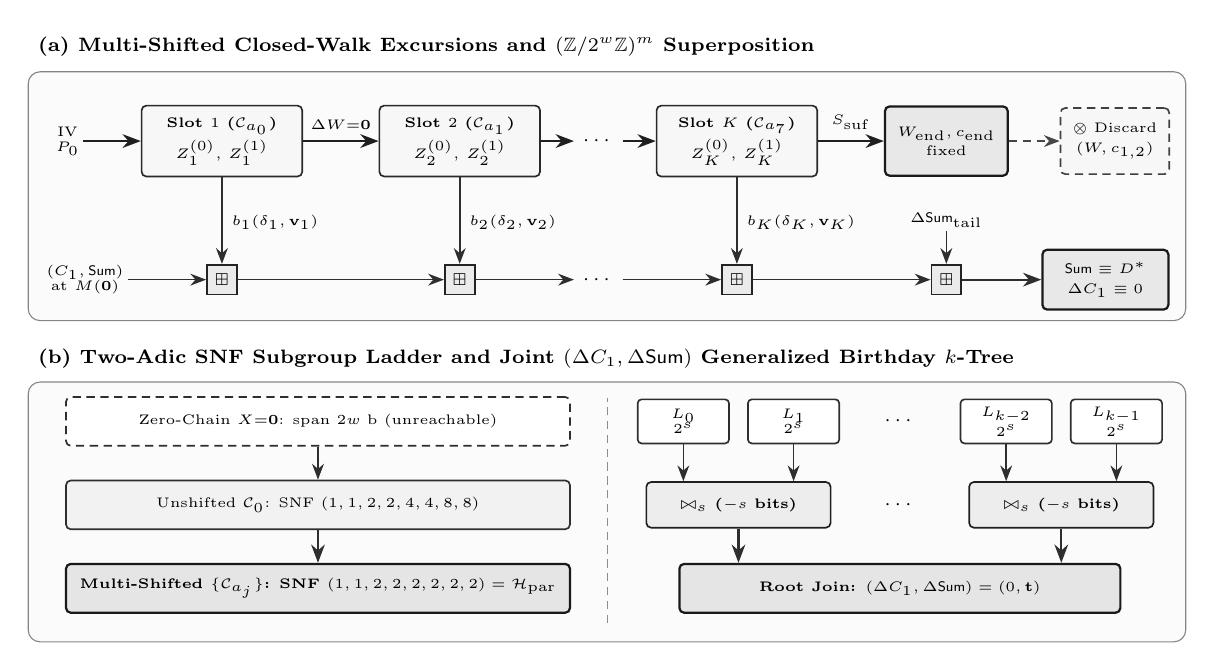
\begin{tikzpicture}[
    >=Stealth,
    slotb/.style={rectangle, draw=black!84, semithick, rounded corners=0.6mm, fill=white, minimum width=20.4mm, minimum height=9.0mm, inner sep=2pt, font=\tiny, align=center},
    addg/.style={rectangle, draw=black!86, semithick, fill=gray!16, minimum size=3.8mm, inner sep=0pt, font=\tiny\bfseries},
    snfrow/.style={rectangle, draw=black!82, semithick, rounded corners=0.6mm, fill=white, minimum width=64.0mm, minimum height=6.2mm, inner xsep=2pt, inner ysep=1.5pt, font=\tiny, align=center},
    leaf/.style={rectangle, draw=black!82, semithick, rounded corners=0.5mm, fill=white, minimum width=11.6mm, minimum height=5.6mm, inner sep=1.4pt, font=\tiny, align=center},
    mnode/.style={rectangle, draw=black!88, semithick, rounded corners=0.6mm, fill=gray!14, minimum width=23.4mm, minimum height=5.8mm, inner sep=1.5pt, font=\tiny\bfseries, align=center},
    wire/.style={->, semithick, draw=black!82},
    zwire/.style={->, thick, draw=black!88},
    dwire/.style={->, semithick, densely dashed, draw=black!72},
    lbl/.style={font=\scriptsize, inner xsep=3pt, inner ysep=1.5pt},
    tlbl/.style={font=\tiny, inner sep=1.4pt}
]

% ================= PANEL (a): ORTHOGONAL TRUNK EXCURSIONS & MODULAR SUPERPOSITION =================
\node[font=\scriptsize\bfseries, anchor=west] at (0.00, 5.44) {(a) Multi-Shifted Closed-Walk Excursions and $(\Zmod{w})^m$ Superposition};

\begin{scope}[on background layer]
    \draw[rounded corners=1.5mm, draw=black!48, fill=gray!3] (0.00, 1.96) rectangle (14.70, 5.12);
\end{scope}

% Upper Trunk Trajectory (y = 4.24)
\node[tlbl, align=center] (iv) at (0.50, 4.24) {\textbf{$\mathrm{IV}$}\\[-0.5pt]$P_0$};
\node[slotb, fill=gray!6] (sl1) at (2.46, 4.24) {\textbf{Slot $1$ ($\mathcal{C}_{a_0}$)}\\[1pt]$Z_1^{(0)},\, Z_1^{(1)}$};
\node[slotb, fill=gray!6] (sl2) at (5.48, 4.24) {\textbf{Slot $2$ ($\mathcal{C}_{a_1}$)}\\[1pt]$Z_2^{(0)},\, Z_2^{(1)}$};
\node[lbl] (sld) at (7.24, 4.24) {$\cdots$};
\node[slotb, fill=gray!6] (slk) at (9.00, 4.24) {\textbf{Slot $K$ ($\mathcal{C}_{a_7}$)}\\[1pt]$Z_K^{(0)},\, Z_K^{(1)}$};
\node[rectangle, draw=black!90, thick, rounded corners=0.6mm, fill=gray!18, minimum width=15.6mm, minimum height=8.8mm, inner sep=1.8pt, font=\tiny\bfseries, align=center] (wend) at (11.66, 4.24) {$W_{\mathrm{end}}, c_{\mathrm{end}}$\\[1pt]{\normalfont\tiny fixed}};
\node[rectangle, draw=black!75, semithick, densely dashed, rounded corners=0.6mm, fill=gray!6, minimum width=13.8mm, minimum height=8.4mm, inner sep=1.5pt, font=\tiny, align=center] (disc) at (13.80, 4.24) {$\otimes$ Discard\\[1pt]$(W, c_{1,2})$};

\draw[zwire] (iv.east)   -- (sl1.west);
\draw[zwire] (sl1.east)  -- node[tlbl, above=2.5pt] {$\Delta W{=}\mathbf{0}$} (sl2.west);
\draw[zwire] (sl2.east)  -- (sld.west);
\draw[zwire] (sld.east)  -- (slk.west);
\draw[zwire] (slk.east)  -- node[tlbl, above=2.5pt] {$S_{\mathrm{suf}}$} (wend.west);
\draw[dwire] (wend.east) -- (disc.west);

% Lower Accumulator & Checksum Bus (y = 2.48)
\node[tlbl, align=center] (base) at (0.72, 2.48) {$(C_1, \SumAcc)$\\[-0.5pt]at $M(\mathbf{0})$};
\node[addg] (ad1) at (2.46, 2.48) {$\boxplus$};
\node[addg] (ad2) at (5.48, 2.48) {$\boxplus$};
\node[lbl]  (add) at (7.24, 2.48) {$\cdots$};
\node[addg] (adk) at (9.00, 2.48) {$\boxplus$};
\node[addg] (adt) at (11.66, 2.48) {$\boxplus$};
\node[rectangle, draw=black!90, thick, rounded corners=0.6mm, fill=gray!18, minimum width=16.0mm, minimum height=7.6mm, inner sep=1.8pt, font=\tiny\bfseries, align=center] (dout) at (13.68, 2.48) {$\SumAcc \equiv D^*$\\[1pt]$\Delta C_1 \equiv 0$};

\draw[wire] (base.east) -- (ad1.west);
\draw[wire] (ad1.east)  -- (ad2.west);
\draw[wire] (ad2.east)  -- (add.west);
\draw[wire] (add.east)  -- (adk.west);
\draw[wire] (adk.east)  -- (adt.west);
\draw[wire, thick] (adt.east) -- (dout.west);

% Deposit taps from slots down to \boxplus gates + tail offset
\draw[wire] (sl1.south) -- node[tlbl, right=2pt, pos=0.52] {$b_1(\delta_1, \mathbf{v}_1)$} (ad1.north);
\draw[wire] (sl2.south) -- node[tlbl, right=2pt, pos=0.52] {$b_2(\delta_2, \mathbf{v}_2)$} (ad2.north);
\draw[wire] (slk.south) -- node[tlbl, right=2pt, pos=0.52] {$b_K(\delta_K, \mathbf{v}_K)$} (adk.north);
\node[tlbl] (toff) at (11.66, 3.24) {$\Delta\SumAcc_{\mathrm{tail}}$};
\draw[wire] (toff.south) -- (adt.north);

% ================= PANEL (b): 2-ADIC SNF LADDER & JOINT WAGNER k-TREE =================
\node[font=\scriptsize\bfseries, anchor=west] at (0.00, 1.48) {(b) Two-Adic SNF Subgroup Ladder and Joint $(\Delta C_1, \Delta\SumAcc)$ Generalized Birthday $k$-Tree};

\begin{scope}[on background layer]
    \draw[rounded corners=1.5mm, draw=black!48, fill=gray!3] (0.00, -2.12) rectangle (14.70, 1.18);
\end{scope}

% Left Half (x = 0.28..7.08): 2-Adic SNF Subgroup Saturation Ladder
\node[snfrow, densely dashed] (r1) at (3.68, 0.68)
    {Zero-Chain $X{=}\mathbf{0}$: span $2w$~b (unreachable)};
\node[snfrow, fill=gray!10] (r2) at (3.68, -0.38)
    {Unshifted $\mathcal{C}_0$: SNF $(1,1,2,2,4,4,8,8)$};
\node[snfrow, fill=gray!20, draw=black!90, thick] (r3) at (3.68, -1.44)
    {\textbf{Multi-Shifted $\{\mathcal{C}_{a_j}\}$: SNF $(1,1,2,2,2,2,2,2) = \Hpar$}};

\draw[wire] (r1.south) -- (r2.north);
\draw[wire, thick] (r2.south) -- (r3.north);

% Vertical divider
\draw[densely dashed, draw=black!45] (7.36, -1.88) -- (7.36, 0.98);

% Right Half (x = 7.64..14.48): Joint (Delta C_1, Delta Sum) Wagner k-Tree (pure vertical alignment)
\node[leaf] (l0) at (8.32,  0.68) {$L_0$\\[-0.5pt]$2^s$};
\node[leaf] (l1) at (9.72,  0.68) {$L_1$\\[-0.5pt]$2^s$};
\node[lbl]  (ld) at (11.07, 0.68) {$\cdots$};
\node[leaf] (l2) at (12.42, 0.68) {$L_{k-2}$\\[-0.5pt]$2^s$};
\node[leaf] (l3) at (13.82, 0.68) {$L_{k-1}$\\[-0.5pt]$2^s$};

\node[mnode] (m0) at (9.02,  -0.38) {$\bowtie_s$ ($-s$~bits)};
\node[lbl]   (md) at (11.07, -0.38) {$\cdots$};
\node[mnode] (m1) at (13.12, -0.38) {$\bowtie_s$ ($-s$~bits)};

\node[rectangle, draw=black!90, thick, rounded corners=0.6mm, fill=gray!20, minimum width=56.0mm, minimum height=6.2mm, inner sep=2pt, font=\tiny\bfseries, align=center] (root) at (11.07, -1.44)
    {Root Join: $(\Delta C_1, \Delta\SumAcc) = (0, \mathbf{t})$};

\draw[wire] (l0.south) -- (l0.south |- m0.north);
\draw[wire] (l1.south) -- (l1.south |- m0.north);
\draw[wire] (l2.south) -- (l2.south |- m1.north);
\draw[wire] (l3.south) -- (l3.south |- m1.north);
\draw[wire, thick] (m0.south) -- (m0.south |- root.north);
\draw[wire, thick] (m1.south) -- (m1.south |- root.north);

\end{tikzpicture}
\caption{Multi-shifted closed-walk preimage architecture over $(\Zmod{w})^m$. \textbf{(a)}~Equal-length closed-walk pairs $(Z_j^{(0)}, Z_j^{(1)})$ across $8$ shifted clean subspaces re-merge on $(W, c_1, c_2)$ at every anchor so $(W_{\mathrm{end}}, c_{\mathrm{end}})$ and the post-message padding and checksum rounds add a fixed constant $\Delta\SumAcc_{\mathrm{tail}}$ before $(W, c_1, c_2)$ is discarded. \textbf{(b)}~Odd $2$-adic units $-\!(2a_j+1)$ collapse the SNF defect to $\Hpar$, and a joint $(\Delta C_1, \Delta\SumAcc)$ Wagner $k$-tree hits $D^*$.}
\label{fig:dsos-preimage}
\end{figure}

\begin{table}[t]
\centering
\caption{First- and second-preimage complexity comparison across all four NIST Blender variants: Blender-$224$ ($w{=}32, m{=}7$), Blender-$256$ ($w{=}32, m{=}8$), Blender-$384$ ($w{=}64, m{=}6$), and Blender-$512$ ($w{=}64, m{=}8$).}
\label{tab:preimage-comp}
\footnotesize
\setlength{\tabcolsep}{3.4pt}
\renewcommand{\arraystretch}{1.05}
\begin{tabular}{@{}llrrrl@{}}
\toprule
\textbf{Variant} & \textbf{Method} & \textbf{Time} & \textbf{Memory} & \textbf{Words} & \textbf{Mechanism} \\
\midrule
Blender-$224$ & Newbold~\cite{New08} & $2^{135.81}$ & $O(n^2)$ & $O(n^2)$ & Joux + checksum birthday \\
Blender-$224$ & Lamberger--Mendel~\cite{Men08,LM09} & $\mathbf{2^{119.81}}$ & $O(n)^{\mathrm{a}}$ & $1{,}121$ & $5$-word sum-fixed Joux \\
\midrule
Blender-$256$ & Newbold~\cite{New08} & $2^{152.00}$ & $O(n^2)$ & $O(n^2)$ & Joux + checksum birthday \\
Blender-$256$ & Lamberger--Mendel~\cite{Men08,LM09} & $2^{136.00}$ & $O(n)^{\mathrm{a}}$ & $1{,}281$ & $5$-word sum-fixed Joux \\
Blender-$256$ & Kl\'{i}ma (single)~\cite{Kli09} & $\ge 2^{107.32}$ & $2^{65.00}$ & $2^{107.32}$ & Odd-lane fixpoint winding \\
Blender-$256$ & Kl\'{i}ma ($2^{2n}$-multi)~\cite{Kli09} & $\ge 2^{171.30}$ & $2^{65.00}$ & $2^{171.30}$ & Odd-lane fixpoint winding \\
Blender-$256$ & Ours (Winding) & $2^{45.46}$ & $2^{18.00}$ & $2^{45.46}$ & $8$-shifted $\Hpar$ + $2$-adic solve \\
Blender-$256$ & \textbf{Ours ($k$-Tree)} & $\mathbf{2^{35.93}}$ & $2^{21.69\mathrm{b}}$ & $2^{27.46}$ & $8$-shifted $\Hpar$ + Wagner $2^{12}$ \\
\midrule
Blender-$384$ & Newbold~\cite{New08} & $2^{232.58}$ & $O(n^2)$ & $O(n^2)$ & Joux + checksum birthday \\
Blender-$384$ & Lamberger--Mendel~\cite{Men08,LM09} & $2^{200.58}$ & $O(n)^{\mathrm{a}}$ & $1{,}921$ & $5$-word sum-fixed Joux \\
Blender-$384$ & Kl\'{i}ma (single)~\cite{Kli09} & $\ge 2^{171.90}$ & $2^{97.00}$ & $2^{171.90}$ & Odd-lane fixpoint winding \\
Blender-$384$ & Kl\'{i}ma ($2^{2n}$-multi)~\cite{Kli09} & $\ge 2^{267.30}$ & $2^{97.00}$ & $2^{267.30}$ & Odd-lane fixpoint winding \\
Blender-$384$ & Ours (Winding) & $2^{89.17}$ & $2^{34.00}$ & $2^{89.17}$ & $8$-shifted $\Hpar$ + $2$-adic solve \\
Blender-$384$ & \textbf{Ours ($k$-Tree)} & $\mathbf{2^{66.34}}$ & $2^{29.60\mathrm{b}}$ & $2^{38.91}$ & $8$-shifted $\Hpar$ + Wagner $2^{14}$ \\
\midrule
Blender-$512$ & Newbold~\cite{New08} & $2^{297.00}$ & $O(n^2)$ & $O(n^2)$ & Joux + checksum birthday \\
Blender-$512$ & Lamberger--Mendel~\cite{Men08,LM09} & $2^{265.00}$ & $O(n)^{\mathrm{a}}$ & $2{,}561$ & $5$-word sum-fixed Joux \\
Blender-$512$ & Kl\'{i}ma (single)~\cite{Kli09} & $\ge 2^{204.32}$ & $2^{129.00}$ & $2^{204.32}$ & Odd-lane fixpoint winding \\
Blender-$512$ & Kl\'{i}ma ($2^{2n}$-multi)~\cite{Kli09} & $\ge 2^{331.30}$ & $2^{129.00}$ & $2^{331.30}$ & Odd-lane fixpoint winding \\
Blender-$512$ & Ours (Winding) & $2^{89.46}$ & $2^{34.00}$ & $2^{89.46}$ & $8$-shifted $\Hpar$ + $2$-adic solve \\
Blender-$512$ & \textbf{Ours ($k$-Tree)} & $\mathbf{2^{67.64}}$ & $2^{38.00\mathrm{b}}$ & $2^{39.25}$ & $8$-shifted $\Hpar$ + Wagner $2^{14}$ \\
\bottomrule
\addlinespace[2pt]
\multicolumn{6}{@{}l@{}}{\scriptsize $^{\mathrm{a}}$Memoryless MITM~\cite{QD89} ($2^{n/2}$ with table lookup).\quad $^{\mathrm{b}}$Single-list size $2^s = 2^{B/(\ell+1)}$.}
\end{tabular}
\end{table}

\section{Architectural Diagnosis and Experimental Evaluation}
\label{sec:eval}

\subsection{Diagnosis of Structural Weaknesses}
\label{subsec:diagnosis}
Our three attacks trace back to three interacting architectural flaws in Blender's ARX-plus-accumulator design, each pointing to a concrete design principle:
\begin{enumerate}[leftmargin=2em]
    \item \textbf{Uniform Stride-$t$ Mask Broadcasting Across $m$ Lanes:} Injecting only $t = 2$ masks alternately across $m \in \{6, 8\}$ words creates $m - t$ linear mask-free XOR chains $X_i = W_i \oplus W_{i+t}$ that close periodically whenever $t \mid m$ and $W_0 \in \{x, \neg x\}$ (Theorem~\ref{thm:divisibility}). Breaking this symmetry requires either distinct round-dependent rotations per lane or coprime tap schedules coupled with wide non-linear state diffusion.
    \item \textbf{Rotation-Sum Compensation Across Discrete Carry-Selected Rotations:} Coupling $(c'_1, c'_2)$ to $r = 8 - (c'_1 + c'_2) \in \{6, 7, 8\}$ allows a $2$-bit carry jump $(0,0) \leftrightarrow (1,1)$ at step~$p$ to be canceled inside the pre-rotation sum ($\rol_2(u)$ and $\ror_2(v)$) with probability $(7/48)^2 \approx 2^{-5.56}$. That carry difference is then healed deterministically at step~$p+1$ via $(2^{w-1}, 2^{w-1} - 1)$ complement inputs (Theorem~\ref{thm:healing-rigidity}). Mixing carries back into multiple non-aligned bit positions and applying at least $4$ rounds of feed-forward state mixing per absorbed message word prevents $2$-step local healing.
    \item \textbf{Unidirectional Accumulator Without Working-State Feed-Forward at Output:} Updating $\SumAcc$ without feeding $\SumAcc$ back into $W$, and discarding $(W, c_1, c_2)$ immediately after the checksum rounds, makes finalization an invariant affine translation (Proposition~\ref{prop:c-inv-zero}). Every closed walk on $(W, c_1, c_2)$ then acts as an exact abelian translation in $(\Zmod{w})^m$. Bijectively mixing $\SumAcc$ and $W$ during finalization and absorbing step counters into every compression round eliminates commuting closed walks and forces non-linear finalization inversion.
\end{enumerate}

\subsection{Experimental Verification and Benchmarks}
\label{subsec:benchmarks}
All solvers and witnesses were implemented in portable C (POSIX threads) and Python~3 without external SAT/SMT or third-party library dependencies. Every output witness was verified byte-for-byte against Bradbury's unmodified NIST SHA-3 Round-1 C reference implementation~\cite{Bra08} on an Apple Silicon workstation:
\begin{enumerate}[leftmargin=2em]
    \item \textbf{Subspace Cycle-Swap Standard-IV Collisions and Multicollisions:} Our $8$-thread overlapping ancestor cycle-swap solver finds verified $16{,}000$-byte ($4{,}000$-word) standard-IV Blender-$256$ collisions in $0.045$~s on a fast seed and $0.731$~s mean ($0.774$~s median, $0.181$~s min, $1.422$~s max) across $10$ independent cold seeds, exploring a mean of $2^{22.6}$ clean DFS nodes. From a single $(P, U, V)$ witness, all $\binom{6}{3} = 20$ balanced $40{,}896$-byte multicollisions were hashed through the official C reference, all producing the identical digest \texttt{8b07ac88b949ef7d3e946af12c79c651c2b7b33d7f1dd09cb7ea0c3836b3b71b}. Empirical out-degree audits across $2{,}000$ uniform clean states per variant measured $2.016, 2.006,$ and $2.010$ on Blender-$256, -384,$ and $-512$, matching Proposition~\ref{prop:outdegree} ($2.000$).
    \item \textbf{All-Variant Closed-Form SFS ($80{,}000 / 80{,}000$ Verified):} Across $20{,}000$ random seeds per variant ($80{,}000$ pairs in total), our deterministic closed-form SFS generator (Theorem~\ref{thm:sfs-all}) succeeded on $100\%$ of seeds with zero retries. It generated pairs in $0.027~\mu$s (Blender-$224$, $113$~B), $0.006~\mu$s (Blender-$256$, $113$~B), $0.054~\mu$s (Blender-$384$, $229$~B), and $0.014~\mu$s (Blender-$512$, $229$~B), all verified against the official C reference.
    \item \textbf{Global-Minimum $24$-Byte Standard-IV and $36$/$40$-Byte Identical-Prefix Collisions:} Table~\ref{tab:short-witnesses} lists our verified short colliding message pairs on full Blender-$256$. Our pure-C $4$-round lane-invariant and $2$-round byte-lattice solver ($0.11\text{--}0.29$~ms per $2$-round inversion) solved $10/10$ cold seeds for $24$-byte standard-IV collisions in $34.58$~s mean on $10$ threads ($1.63$~s min; $0.057$~s single-thread best). It also solved a $40$-byte identical-prefix collision for the $16$-byte ASCII prefix \texttt{"Dear Bob, wire \$"} in $145.5$~s on $10$ threads ($42$ two-round targets), alongside a $36$-byte ($3$-round steered) identical-prefix witness for the same prefix.
    \item \textbf{Verification of $2$-Adic SNF Ranks and Closed-Walk Modular Superposition:} Across $500$ independent closed-walk slots per configuration on the official C reference, empirical $2$-adic Smith Normal Form decomposition confirmed the exact subgroup invariant factors $(1, 1, 2, 2, 4, 4, 8, 8)$ (index $2^{12}$) in the unshifted subspace $\mathcal{C}_0$ and $(1, 1, 2, 2, 2, 2, 2, 2)$ (index $2^6$, matching $\Hpar$) across $4$ and $8$ shifted subspaces $\mathcal{C}_{a_j}$ (Theorem~\ref{thm:snf-hierarchy}). We also confirmed $100\%$ exact modular superposition and post-message finalization invariance (Proposition~\ref{prop:c-inv-zero}) across end-to-end $8$-anchor closed-walk families satisfying $\Delta C_1 \equiv 0 \pmod{2^{32}}$ on the unmodified NIST C reference.
\end{enumerate}

\begin{table}[t]
\centering
\caption{Verified minimal-length standard-IV ($24$~B) and identical-prefix ($36$~B and $40$~B, ASCII prefix ``\texttt{Dear Bob, wire }\$'') colliding pairs for full Blender-$256$ on the official NIST C reference~\cite{Bra08}.}
\label{tab:short-witnesses}
\scriptsize
\setlength{\tabcolsep}{3.5pt}
\begin{tabular}{@{}ll@{}}
\toprule
\textbf{Item} & \textbf{Verified Hexadecimal Value} \\
\midrule
\multicolumn{2}{@{}l}{\textbf{$24$-Byte ($6$-Word) Standard-IV Collision Pair A}} \\
$M_1$ & \texttt{66b2d21e26d2d06c6eb3e7e2f5e97fe5e367af98dfff7fc1} \\
$M_2$ & \texttt{66b2d21e26d2d06c6eb3e7e2f5e97fe5a267af1b2000803e} \\
Digest & \texttt{3dab8fdaf25bc778e60ea5c22b332f57875003724fb29615aedbf749fde750ee} \\
\midrule
\multicolumn{2}{@{}l}{\textbf{$24$-Byte ($6$-Word) Standard-IV Collision Pair B}} \\
$M_1$ & \texttt{2d0f9baed58c8332feaed2c6274dfa3eccca0d99b31c8466} \\
$M_2$ & \texttt{2d0f9baed58c8332feaed2c6274dfa3e330416664ce37b99} \\
Digest & \texttt{4dbdaf9d59fbdac4f0721cfd96a6eaa6cf7da4b0e72ef6d7516c931233c03ff5} \\
\midrule
\multicolumn{2}{@{}l}{\textbf{$36$-Byte ($9$-Word) Identical-Prefix Collision Pair$^{\mathrm{a}}$}} \\
$M_1$ & \texttt{4465617220426f622c207769726520243b3b0c1861f200be53811121852bbf00efd219c2} \\
$M_2$ & \texttt{4465617220426f622c207769726520243b3b0c1861f200be5381112164d1f284102de63d} \\
Digest & \texttt{6b6c36da8ad5f932d384394af95eadf64de470977245367e3fa168ac835fd2b2} \\
\midrule
\multicolumn{2}{@{}l}{\textbf{$40$-Byte ($10$-Word) Identical-Prefix Collision Pair$^{\mathrm{a}}$}} \\
$M_1$ & \texttt{4465617220426f622c20776972652024b89c419ad38fd20e65c9a79c84bd45f046bb10bae0fef7bf} \\
$M_2$ & \texttt{4465617220426f622c20776972652024b89c419ad38fd20e65c9a79c84bd45f007b9003a1f010840} \\
Digest & \texttt{8d5ee26f516017afe572029ec9fa75ee9b242a9a27cc73a2e4cec873578da3f8} \\
\bottomrule
\end{tabular}
\par\smallskip
{\scriptsize $^{\mathrm{a}}$ Both pairs start with the $16$-byte ASCII prefix \texttt{"Dear Bob, wire \$"} (\texttt{4465617220426f622c20776972652024}).}
\end{table}

\paragraph{Use of AI.}
The cryptanalytic results and artifacts were initially developed through an autonomous agent system powered by a MiniMax internal model. We validated the key technical claims and refined the presentation of the manuscript.

{\emergencystretch=1.5em
\begin{thebibliography}{99}

\bibitem{Bra08}
C.~Bradbury,
``BLENDER: A Proposed New Family of Cryptographic Hash Algorithms,'' Algorithm Specification and Supporting Documentation, Submission to the NIST SHA-3 Competition (Round~1), Oct.~2008.

\bibitem{CJ98}
F.~Chabaud and A.~Joux,
``Differential Collisions in SHA-0,'' in \emph{Advances in Cryptology -- CRYPTO'98}, LNCS, vol.~1462, pp.~56--71, Springer, 1998.

\bibitem{DC98}
J.~Daemen and C.~Clapp,
``Fast Hashing and Stream Encryption with PANAMA,'' in \emph{Fast Software Encryption -- FSE'98}, LNCS, vol.~1372, pp.~60--74, Springer, 1998.

\bibitem{GK08}
P.~Gauravaram and J.~Kelsey,
``Linear-XOR and Additive Checksums Don't Protect Damg\aa rd--Merkle Hashes from Generic Attacks,'' in \emph{Topics in Cryptology -- CT-RSA~2008}, LNCS, vol.~4964, pp.~36--51, Springer, 2008.

\bibitem{Hat08}
B.~Hattersley,
``Waterfall Hash --- Algorithm Specification and Analysis,'' Version~1.0, Submission to the NIST SHA-3 Competition (Round~1), Oct.~2008.

\bibitem{Jou04}
A.~Joux,
``Multicollisions in Iterated Hash Functions. Application to Cascaded Construc\-tions,'' in \emph{Advances in Cryptology -- CRYPTO~2004}, LNCS, vol.~3152, pp.~306--316, Springer, 2004.

\bibitem{KK06}
J.~Kelsey and T.~Kohno,
``Herding Hash Functions and the Nostradamus Attack,'' in \emph{Advances in Cryptology -- EUROCRYPT~2006}, LNCS, vol.~4004, pp.~183--200, Springer, 2006.

\bibitem{Kli08}
V.~Kl\'{i}ma,
``A Near-Collision Attack on BLENDER-256,'' Public Comment to the NIST SHA-3 Competition (Round~1), Dec.~2008.

\bibitem{Kli09}
V.~Kl\'{i}ma,
``Huge Multicollisions and Multipreimages of Hash Functions BLENDER-n,'' Cryptology ePrint Archive, Paper 2009/006, Jan.~2009.

\bibitem{LM09}
M.~Lamberger and F.~Mendel,
``Structural Attacks on Two SHA-3 Candidates: Blender-n and DCH-n,'' in \emph{Information Security -- ISC~2009}, LNCS, vol.~5735, pp.~68--78, Springer, 2009.

\bibitem{Men08}
F.~Mendel,
``Preimage Attack on Blender,'' Unpublished note, ECRYPT SHA-3 Zoo, Dec.~2008. \url{https://ehash.isec.tugraz.at/uploads/4/48/Blender-preimage.pdf}.

\bibitem{MPRKS08}
F.~Mendel, N.~Pramstaller, C.~Rechberger, M.~Kontak, and J.~Szmidt,
``Cryptanalysis of the GOST Hash Function,'' in \emph{Advances in Cryptology -- CRYPTO~2008}, LNCS, vol.~5157, pp.~162--178, Springer, 2008.

\bibitem{New08}
C.~Newbold,
``Observations and Attacks On The SHA-3 Candidate Blender,'' Unpublished note, ECRYPT SHA-3 Zoo, Dec.~2008. \url{https://ehash.isec.tugraz.at/uploads/2/20/Observations_on_Blender.pdf}.

\bibitem{QD89}
J.-J.~Quisquater and J.-P.~Delescaille,
``How Easy is Collision Search? New Results and Applications to DES,'' in \emph{Advances in Cryptology -- CRYPTO'89}, LNCS, vol.~435, pp.~408--413, Springer, 1990.

\bibitem{NIST09}
A.~Regenscheid, R.~Perlner, S.-j.~Chang, J.~Kelsey, M.~Nandi, and S.~Paul,
``Status Report on the First Round of the SHA-3 Cryptographic Hash Algorithm Competition,'' NIST Interagency Report (NISTIR)~7620, National Institute of Standards and Technology, Sept.~2009.

\bibitem{SLdW07}
M.~Stevens, A.~K.~Lenstra, and B.~de~Weger,
``Chosen-Prefix Collisions for MD5 and Colliding X.509 Certificates for Different Identities,'' in \emph{Advances in Cryptology -- EUROCRYPT~2007}, LNCS, vol.~4515, pp.~1--22, Springer, 2007.

\bibitem{Wag02}
D.~Wagner,
``A Generalized Birthday Problem,'' in \emph{Advances in Cryptology -- CRYPTO~2002}, LNCS, vol.~2442, pp.~288--304, Springer, 2002.

\bibitem{WY05}
X.~Wang and H.~Yu,
``How to Break MD5 and Other Hash Functions,'' in \emph{Advances in Cryptology -- EUROCRYPT~2005}, LNCS, vol.~3494, pp.~19--35, Springer, 2005.

\bibitem{XL08}
L.~Xu and J.~Li,
``Semi-free start collision attack on Blender,'' Cryptology ePrint Archive, Paper 2008/532, Dec.~2008.

\end{thebibliography}
}

\end{document}
